\documentclass[11pt,a4paper]{article}

\usepackage[margin=22mm]{geometry}
\usepackage[T1]{fontenc}
\usepackage[utf8]{inputenc}
\usepackage{lmodern}
% The previous report was typeset in Linux Libertine. To use the same font, install the
% MiKTeX package "libertine" (or compile on Overleaf) and uncomment the next line.
% \usepackage{libertine}
\usepackage{microtype}
\usepackage{amsmath,amssymb}
\usepackage{graphicx}
\usepackage{booktabs}
\usepackage{longtable}
\usepackage{array}
\usepackage{tabularx}
\usepackage{xcolor}
\usepackage{float}
\usepackage{caption}
\usepackage{subcaption}
\usepackage{fancyhdr}
\usepackage{enumitem}
\usepackage{hyperref}

% All figures are read directly from the final_report folders.
\graphicspath{{../}}
\hypersetup{
  colorlinks=true,
  linkcolor=blue!45!black,
  citecolor=blue!45!black,
  urlcolor=blue!55!black,
  pdftitle={Explaining BERT, CLIP Text and CLIP Vision with Partition SHAP},
  pdfauthor={Mohsin Gourab}
}
\captionsetup{font=small,labelfont=bf}
\captionsetup[sub]{font=footnotesize}
\setlength{\parindent}{0pt}
\setlength{\parskip}{0.6em}
\setcounter{secnumdepth}{3}
\setcounter{tocdepth}{2}
\emergencystretch=2em
\renewcommand{\arraystretch}{1.12}

\pagestyle{fancy}
\fancyhf{}
\fancyhead[L]{BERT and CLIP explanations with Partition SHAP}
\fancyhead[R]{TRDP II}
\fancyfoot[C]{\thepage}
\setlength{\headheight}{14pt}

\newcolumntype{Y}{>{\raggedright\arraybackslash}X}
\newcommand{\up}{$\uparrow$}
\newcommand{\down}{$\downarrow$}

% One page with the five SHAP plots of one sentence and one model.
% [#1] size factor (smaller for the first page of an appendix, which also holds the
% section heading), #2 folder, #3 sentence id, #4 model name, #5 label prefix
\newcommand{\sentenceplots}[5][1]{%
  \begin{figure}[H]
    \centering
    \begin{subfigure}{\textwidth}\centering
      \includegraphics[width=\textwidth,height=#1\dimexpr0.28\textheight\relax,keepaspectratio]{#2/#3/#3_dual_class_word_bar.pdf}
      \caption{Word-level SHAP bars for the NEG and POS outputs}
    \end{subfigure}\\[1mm]
    \begin{subfigure}{\textwidth}\centering
      \includegraphics[width=\textwidth,height=#1\dimexpr0.28\textheight\relax,keepaspectratio]{#2/#3/#3_presentation_overview.pdf}
      \caption{Presentation overview: word values and sentence summary}
    \end{subfigure}\\[1mm]
    \begin{subfigure}[t]{0.32\textwidth}\centering
      \includegraphics[width=\textwidth,height=#1\dimexpr0.21\textheight\relax,keepaspectratio]{#2/#3/#3_token_class_matrix.pdf}
      \caption{Token-by-class matrix}
    \end{subfigure}\hfill
    \begin{subfigure}[t]{0.32\textwidth}\centering
      \includegraphics[width=\textwidth,height=#1\dimexpr0.21\textheight\relax,keepaspectratio]{#2/#3/#3_word_class_matrix.pdf}
      \caption{Word-by-class matrix}
    \end{subfigure}\hfill
    \begin{subfigure}[t]{0.32\textwidth}\centering
      \includegraphics[width=\textwidth,height=#1\dimexpr0.21\textheight\relax,keepaspectratio]{#2/#3/#3_summary_matrix.pdf}
      \caption{Sentence summary matrix}
    \end{subfigure}
    \caption{#4, sentence #3: all five SHAP plots.}
    \label{fig:#5-#3}
  \end{figure}
  \clearpage
}

% Two CLIP vision patch overlays on one page; [#1] size factor as above.
\newcommand{\visionpair}[3][1]{%
  \begin{figure}[H]
    \centering
    \includegraphics[width=0.8\textwidth,height=#1\dimexpr0.41\textheight\relax,keepaspectratio]{04_clip_vision_shap_I1_I10_patch_overlay_values/#2_SHAP_patch_overlay_values.pdf}
    \caption{CLIP vision, image #2: 7$\times$7 patch SHAP values over the 224$\times$224 model input.}
    \label{fig:overlay-#2}
    \vspace{4mm}
    \includegraphics[width=0.8\textwidth,height=#1\dimexpr0.41\textheight\relax,keepaspectratio]{04_clip_vision_shap_I1_I10_patch_overlay_values/#3_SHAP_patch_overlay_values.pdf}
    \caption{CLIP vision, image #3: 7$\times$7 patch SHAP values over the 224$\times$224 model input.}
    \label{fig:overlay-#3}
  \end{figure}
  \clearpage
}

\begin{document}

\hypersetup{pageanchor=false}
\begin{titlepage}
  \centering
  \vspace*{22mm}
  {\Large TRDP II\par}
  \vspace{16mm}
  {\huge\bfseries Explaining BERT, CLIP Text and CLIP Vision\\[2mm] with Partition SHAP\par}
  \vspace{6mm}
  {\Large A qualitative and quantitative evaluation of text and image explanations\par}
  \vspace{24mm}
  {\large Mohsin Gourab\par}
  \vfill
  \begin{minipage}{0.84\textwidth}
    \small
    This report continues our previous report, in which we explained the sentiment
    decisions of a BERT classifier with Partition SHAP. We extend that work in three
    directions: we explain both sentiment outputs instead of a single score, we apply the
    same method to the text and vision encoders of CLIP, and we evaluate all explanations
    with established faithfulness and plausibility metrics. The BERT checkpoint, the
    qualitative sentence set and the label convention of the previous report were kept, and
    all evaluations were computed on top of the stored explanations without changing them.
  \end{minipage}
  \vfill
  {\large 30 September 2026\par}
\end{titlepage}
\hypersetup{pageanchor=true}

\pagenumbering{roman}
\begin{abstract}
In our previous report we applied Partition SHAP to a BERT classifier fine-tuned on
SST-2 and showed that it recovers the expected sentiment words for ten qualitative
sentences. In this report we extend that analysis to three models: the same BERT
classifier, the frozen CLIP text encoder used as a zero-shot sentiment classifier through
prompt prototypes, and the CLIP vision encoder.

We first explain the negative and positive output of BERT and CLIP text for the ten
qualitative sentences (S1--S10). Both models highlight the obvious sentiment words, but
BERT does so with clear margins while CLIP's decisions are very close and partly driven by
neutral words such as \emph{movie} or \emph{film}. We then evaluate the explanations on
500 balanced SST-2 sentences. The explanations of BERT are more faithful than those of
CLIP text (comprehensiveness 0.772 vs.\ 0.705, sufficiency 0.223 vs.\ 0.331, deletion AOPC
0.890 vs.\ $-0.368$) and agree better with human word-level sentiment ratings
(rationale F1 0.494 vs.\ 0.350, using the Stanford Sentiment Treebank word ratings as a
proxy reference). For CLIP vision on ten images, removing the highest-ranked patches
quickly lowers the similarity to the original image embedding (deletion AUC 0.711,
insertion AUC 0.849, AOPC 0.199), and the highest-ranked patch lies on the main object in
9 of 10 images (7 of 10 without a pixel tolerance). All explanations reproduce the
explained model outputs up to floating-point precision. We discuss how the masking
baseline, the very small CLIP decision margins and the proxy references limit how far
these numbers can be interpreted.
\end{abstract}

\clearpage
\tableofcontents
\listoffigures
\listoftables
\clearpage
\pagenumbering{arabic}

% ======================================================================
\section{Introduction}

The goal of our TRDP work is to understand \emph{which parts of the input} a model uses
when it makes a decision. For a sentiment classifier these are the words that make a
review positive or negative; for an image model they are the regions of the picture.
An explanation of this kind is only useful if it really reflects the model, so an
important part of the work is to check the explanations and not only to look at them.

In our previous report we explained a BERT classifier fine-tuned on SST-2 with Partition
SHAP~\cite{lundberg2017}. SHAP does not look inside the network. It asks a counterfactual
question instead: how does the model output change when some words are hidden and others
remain visible? We explained the difference between the positive and the negative logit
for ten qualitative sentences (S1--S10). All ten predictions were correct, the base value
plus the SHAP values reconstructed the margin exactly, and the strongest attributions went
to clear sentiment words such as \emph{beautiful}, \emph{outstanding}, \emph{boring},
\emph{weak} and \emph{captivating}. Masking the highest-ranked words lowered the decision
score by 5.31 logits on average, while keeping only those words lost 0.89 logits.

That report left three questions open. First, it explained only one number, the margin
between the two classes, so it did not show how each word acts on the NEG and on the POS
output. Second, it covered only one model. Third, its faithfulness test used only ten
sentences and raw logit values, which cannot be compared across models. The objectives of
the present report are therefore:

\begin{enumerate}[label=(\arabic*)]
  \item to explain the NEG and the POS output of BERT separately and to relate the result
        to the margin explanation of the previous report;
  \item to apply the same procedure to the CLIP text encoder~\cite{radford2021}, used as a
        zero-shot sentiment classifier through prompts, and to compare its explanations
        with those of BERT;
  \item to measure the faithfulness of the BERT and CLIP text explanations on 500 SST-2
        sentences with comprehensiveness, sufficiency and deletion AOPC;
  \item to measure how well the words selected by SHAP agree with human word-level
        sentiment (token-level rationale precision, recall and F1);
  \item to explain the CLIP vision encoder at the level of image patches and to evaluate
        these explanations with deletion and insertion AUC, AOPC and the pointing game.
\end{enumerate}

An important principle throughout the project was that the evaluation must not change
the thing it evaluates. The models, datasets, masking procedures and stored SHAP values
of the underlying experiments were reused as they were; the metrics were computed on top
of them, and every evaluation run checked that the source folders were left untouched.

The report is organized as follows. Section~\ref{sec:method} describes the models, the
explanation method and the evaluation measures. Section~\ref{sec:workflow} summarizes the
implementation workflow and Section~\ref{sec:setup} the data and experimental setup.
Section~\ref{sec:results} presents the results, which we discuss in
Section~\ref{sec:discussion} before concluding in Section~\ref{sec:conclusion}. All
sentence-level and image-level plots are collected in the appendices.

% ======================================================================
\section{Model and explanation methodology}\label{sec:method}

\subsection{SHAP and Partition SHAP}

SHAP explains one prediction of a model by distributing the model output over the input
features~\cite{lundberg2017}. A feature can be a word, a sub-word token or an image patch.
To measure the contribution of a feature, SHAP evaluates the model on many
\emph{perturbed} inputs in which some features are hidden. Hidden text tokens are replaced
by a mask token or deleted, and hidden image regions are replaced by a blurred version of
the image. The result is one signed value per feature: a positive value means the
feature increases the explained output, a negative value means it decreases it.

The most useful property of SHAP for our purposes is \emph{additivity}. For every input
$x$ with features $1,\dots,M$ the explanation satisfies
\begin{equation}
  f(x) = \phi_0 + \sum_{i=1}^{M} \phi_i ,
  \label{eq:additivity}
\end{equation}
where $f(x)$ is the explained model output, $\phi_0$ is the \emph{base value} (the output
when all features are hidden) and $\phi_i$ is the contribution of feature $i$. We check
this equation for every explanation in the report; the difference between the two sides
is called the \emph{additivity residual}.

Computing exact Shapley values requires all $2^M$ subsets of features and is too expensive.
As in the previous report, we use the \emph{Partition} explainer of the SHAP
library~\cite{shapdocs}, which groups the features into a hierarchy (neighboring words, or
neighboring image blocks) and only evaluates coalitions that respect this hierarchy. The
resulting values are Owen values, an approximation of Shapley values that still satisfies
Equation~\eqref{eq:additivity}. In all experiments we allowed at most 500 model evaluations
per sentence or image.

\subsection{BERT sentiment classifier}

We use the same checkpoint as in the previous report,
\texttt{textattack/bert-base-uncased-SST-2}~\cite{devlin2019,morris2020}, a BERT-base model
that was already fine-tuned on the binary SST-2 sentiment task~\cite{socher2013,wang2019}.
It outputs two logits, one for the negative (NEG) and one for the positive (POS) class, and
predicts the class with the larger logit. We did not train or fine-tune it further. The
label convention of the previous report is kept: index~0 is NEG and index~1 is POS. This
mapping was re-checked on the ten qualitative sentences before any evaluation.

\subsection{CLIP text encoder as a zero-shot sentiment classifier}

CLIP~\cite{radford2021} is trained to match images with their captions; its text encoder
maps a sentence to an embedding vector. It has no sentiment output, so we turn it into a
zero-shot sentiment classifier. We write a small set of negative prompts (e.g.\ ``This movie
is terrible.'') and positive prompts (e.g.\ ``This movie is excellent.''), embed them, and
average the embeddings per class into a NEG and a POS \emph{prototype}. The NEG and POS
scores of a sentence are its cosine similarities to the two prototypes, and the predicted
class is the one with the higher similarity. These scores are similarities, not
probabilities, and they are typically very close to each other. We use the checkpoint
\texttt{openai/clip-vit-base-patch32} and keep it frozen.

\subsection{CLIP vision encoder}

The vision tower of the same CLIP checkpoint is a Vision Transformer~\cite{dosovitskiy2021}
that splits the $224\times224$ input into $7\times7=49$ patches of $32\times32$ pixels.
Like the text encoder, it outputs an embedding and no class. In our vision experiment the
explained output is therefore image-only: the cosine similarity between the embedding of a
perturbed image and the embedding of the original image. The original image scores exactly
1, and a patch with a large SHAP value is a region that CLIP needs to keep its
representation of the image. No text, prompts or labels are involved.

\subsection{Evaluation of explanations}\label{sec:metrics-background}

An explanation can be evaluated in two different ways~\cite{deyoung2020}.
\emph{Faithfulness} asks whether the explanation reflects what the model actually does:
if we remove the features that the explanation calls important, the model output should
change a lot; if we keep only those features, it should change little. \emph{Plausibility}
asks whether the explanation agrees with what a human would point at, for example the
sentiment words of a review or the object in a photo.

For text we use the faithfulness metrics \emph{comprehensiveness} and \emph{sufficiency}
from the ERASER benchmark~\cite{deyoung2020}, which the previous report already used on ten
sentences, and the \emph{area over the perturbation curve} (AOPC)~\cite{samek2017}. For
plausibility we use \emph{token-level rationale F1}, which compares the selected words with
human-marked words~\cite{deyoung2020}. For images we use the \emph{deletion} and
\emph{insertion} curves of RISE~\cite{petsiuk2018}, AOPC, and the \emph{pointing
game}~\cite{zhang2018}, which checks whether the most important location lies on the
annotated object. The next two subsections describe the exact procedures.

\subsection{Text measures}\label{sec:text-metrics}

All four text measures use the same procedure for BERT and CLIP text, so any difference
comes from the models and not from the evaluation. They are computed for the decision
margin POS$-$NEG, because it is the quantity that decides the prediction (POS if the
margin is positive, NEG otherwise).

\paragraph{Decision score.} Removing a word should be judged from the point of view of the
predicted class. As in the previous report we therefore use the \emph{decision score}
\begin{equation}
  s(x) = \begin{cases}
    \phantom{-}\text{margin}(x) & \text{if the model predicts POS,}\\
    -\text{margin}(x) & \text{if the model predicts NEG,}
  \end{cases}
  \label{eq:decision}
\end{equation}
which is positive for the original sentence and shrinks when evidence for the prediction
is removed.

\paragraph{Ranking and cut-offs.} The content words of a sentence (punctuation excluded)
are ranked by the absolute SHAP value of the margin; ties are broken by position. We then
take the top 10\,\%, 20\,\%, 30\,\% and 50\,\% of the content words (at least one word),
the same fractions as in the previous report. On average this is 2.1, 3.8, 5.5 and 8.6
words.

\paragraph{The measures.}
\begin{itemize}[leftmargin=*]
  \item \textbf{Comprehensiveness (\up).} Delete the top-ranked words and measure how much
        the decision score drops. A large drop means the explanation found words the model
        really needs. We average the drop over the four cut-offs.
  \item \textbf{Sufficiency (\down).} Keep \emph{only} the top-ranked words (and the
        punctuation) and measure how much the decision score drops. A small drop means the
        selected words alone are enough to support the decision. Again averaged over the
        cut-offs.
  \item \textbf{Deletion AOPC (\up).} The same deletions as for comprehensiveness, but each
        drop is divided by the sentence's own decision score before averaging. This is the
        measure of the original 500-sentence experiment, which we reproduce exactly.
  \item \textbf{Token-level rationale precision, recall and F1 (\up).} Compare the
        top-ranked words with a set of reference sentiment words: precision is the share of
        selected words that are reference words, recall is the share of reference words
        that were selected, and F1 combines both. Averaged over the four cut-offs.
\end{itemize}

\paragraph{Making BERT and CLIP comparable.} In the previous report comprehensiveness and
sufficiency were reported in logits, which is fine for one model but not for a comparison.
BERT's margin is measured in logits (on average 6.06), CLIP's in cosine similarity (on
average 0.0046). A raw drop of 1.0 would be huge for CLIP and small for BERT. We therefore
divide comprehensiveness and sufficiency by the model's \emph{average} absolute decision
score over the 500 sentences, so that both measures read as ``share of a typical decision
margin''. Deletion AOPC instead divides by the margin of each individual sentence, as in
the original 500-sentence experiment. This makes a difference for CLIP: 73 of its 500
sentences have a margin below 0.001, and dividing by such a tiny number produces very large
values. We come back to this in Section~\ref{sec:text-results}.

\paragraph{Reference words for rationale F1.} Rationale F1 normally requires humans to
mark the words that justify the label of each sentence. SST-2 does not contain such
rationales, and we did not want to invent them. The Stanford Sentiment
Treebank~\cite{socher2013}, from which SST-2 is derived, does however contain a human
sentiment rating (0 = very negative, 1 = very positive) for every phrase and every single
word. We use these ratings as a \emph{proxy} reference: a content word counts as a
sentiment word if its rating lies outside SST's own neutral interval (0.4, 0.6]. All 8,404
content words of the 500 sentences received a rating, and 1,365 of them are sentiment
words. Thirty-two sentences contain no sentiment word at all; recall is undefined for them,
so they are excluded from the rationale measures for both models (468 sentences remain).
Because the words were rated out of context, this measures agreement with human lexical
sentiment rather than with sentence-specific human rationales.

\subsection{Image measures}\label{sec:vision-metrics}

The image measures reuse the ranking and masking of the vision experiment. The 49 patches
are ranked by their absolute SHAP value (all patch values were non-negative, so this is
the same as the signed ranking). A removed patch is replaced by the blurred image that
SHAP used as its background, so the explanation and its evaluation share one definition
of a ``missing'' region. The fully blurred image scores between 0.30 and 0.56 (mean 0.45),
not zero.

\begin{itemize}[leftmargin=*]
  \item \textbf{Deletion AUC (\down).} Blur the patches one at a time, from the most to the
        least important, and record the similarity after each step. The deletion curve
        starts at 1 (original image) and ends at the fully blurred score. We report the
        area under this curve with the fraction of removed patches on the x-axis. A good
        explanation makes the curve fall early, so a lower area is better.
  \item \textbf{Insertion AUC (\up).} Start from the fully blurred image and restore the
        patches in the same order. A good explanation brings the similarity back to 1
        quickly, so a higher area is better.
  \item \textbf{AOPC (\up).} The average drop in similarity after blurring the top 10, 20,
        30 and 50\,\% of the patches (5, 10, 15 and 25 patches), the same cut-offs as for text.
  \item \textbf{Pointing game (\up).} For each image we check whether the center of the
        highest-ranked patch lies inside a bounding box of the image's main object. The
        accuracy is the share of images with a hit. As in the original
        definition~\cite{zhang2018}, a tolerance of 15 pixels is allowed; we also report the
        strict result without tolerance.
\end{itemize}

The images have no bounding boxes, so we annotated one target object per image ourselves
(Appendix~\ref{app:boxes}). The boxes were drafted by looking only at the images, never at
the SHAP maps, and were then reviewed and approved. They are therefore \emph{author
annotations}, not benchmark ground truth. For scene images such as the crowd at a pool (I2)
or the market stall (I7) we used one box around the group of people. Since the explained
score is image-only, the pointing game here tells us whether the most important patch lies
on the main object, not whether CLIP localizes a named class.

% ======================================================================
\section{Implementation workflow}\label{sec:workflow}

Figure~\ref{fig:workflow} summarizes the path from an input to the evaluated
explanation. It is the same for all three models; only the features, the way hidden
features are represented and the explained output change.

\begin{figure}[htb]
  \centering
  \fbox{\begin{minipage}{0.86\textwidth}
    \centering\small
    Input: a sentence or an image\\[0.5mm]
    $\downarrow$\\[0.5mm]
    Features: WordPiece or BPE tokens, whole words, or $7\times7$ image patches\\[0.5mm]
    $\downarrow$\\[0.5mm]
    SHAP masker $\rightarrow$ hierarchy-consistent coalitions of visible and hidden features\\[0.5mm]
    $\downarrow$\\[0.5mm]
    Hidden features: \texttt{[MASK]} token, deleted word or blurred region\\[0.5mm]
    $\downarrow$\\[0.5mm]
    Frozen model wrapper $\rightarrow$ explained output(s): BERT logits, CLIP text
    similarities or CLIP image similarity\\[0.5mm]
    $\downarrow$\\[0.5mm]
    Partition SHAP $\rightarrow$ one value per feature and output, additivity checked\\[0.5mm]
    $\downarrow$\\[0.5mm]
    Aggregation $\rightarrow$ word-level or patch-level values and plots\\[0.5mm]
    $\downarrow$\\[0.5mm]
    Evaluation $\rightarrow$ faithfulness and plausibility measures on the stored values
  \end{minipage}}
  \caption{Processing sequence followed by the implementation.}
  \label{fig:workflow}
\end{figure}

Each experiment is a separate project with the same structure as in the previous report:
a model wrapper that isolates tokenization or image preprocessing and inference, a module
for masking and aggregation (WordPiece or BPE tokens to words, pixels to patches), a module
for evaluation, a plotting module and a run script that handles configuration, input and
output. The model wrappers evaluate every perturbed input without gradients and with the
model in evaluation mode. Sub-word values are summed into words, and pixel values into
$32\times32$ patches, only after SHAP has computed them; summation keeps
Equation~\eqref{eq:additivity} valid.

The evaluation measures were implemented in two additional projects that read the stored
SHAP values and never write into the original experiment folders. Because the measures
were added to finished experiments, we built several checks into this code. Every run
stops before writing any result if one of them fails:

\begin{itemize}[leftmargin=*]
  \item the stored SHAP values are complete and satisfy additivity;
  \item the rebuilt word or patch ranking and the rebuilt deletion inputs are identical to
        the ones stored by the original experiments;
  \item re-scoring the original inputs and the stored deletion inputs with the frozen
        models reproduces the stored scores (largest difference $1.3\times10^{-5}$ logits
        for BERT and below $10^{-6}$ for CLIP);
  \item the recomputed deletion AOPC equals the value stored by the original 500-sentence
        experiment;
  \item the source folders are hashed before and after each run and must be unchanged.
\end{itemize}

% ======================================================================
\section{Experimental setup}\label{sec:setup}

\subsection{Data}

\paragraph{Qualitative sentence set (S1--S10).} The qualitative set of the previous report
contains ten manually specified sentences, six positive and four negative
(Appendix~\ref{app:sentences}). Several contain mixed evidence, for example S3 (\emph{slow}
vs.\ \emph{outstanding}) and S8 (\emph{weak} vs.\ \emph{captivating}). They are meant for
inspection, not for measuring accuracy.

\paragraph{500 SST-2 sentences.} For the quantitative text experiments we use a fixed,
balanced subset of the SST-2 development set with 250 negative and 250 positive sentences.
The subset was selected earlier in the project (excluding inspected and duplicate
sentences) and was used unchanged; a SHA-256 hash of the file is checked before every run.
Both text models explain exactly the same sentences in the same order.

\paragraph{Ten images (I1--I10).} For the vision experiment we use ten natural photographs,
for example a horse in a field, a kayak on the sea, two puppies and a child on a climbing
net. CLIP resizes each image so that the shorter side is 224 pixels and keeps the central
$224\times224$ crop; only this crop can receive attribution. The images come without any
annotation.

\subsection{Overview of the experiments}

Table~\ref{tab:experiments} summarizes the four experiments of this report. Experiments A
and B are qualitative and explain the two class outputs separately. Experiment C explains
the same 500 sentences with both text models and is the basis of the text measures.
Experiment D explains the ten images.

\begin{table}[htb]
  \centering
  \caption{The four SHAP experiments of this report.}
  \label{tab:experiments}
  \small
  \begin{tabularx}{\textwidth}{@{}l l Y Y Y@{}}
    \toprule
    & Data & Explained output & Features and masking & Evaluation \\
    \midrule
    A & S1--S10 & BERT NEG and POS logits &
        WordPiece tokens replaced by \texttt{[MASK]}; values summed to words &
        additivity, qualitative, comparison with the previous report \\
    B & S1--S10 & CLIP text NEG and POS similarity &
        BPE tokens deleted (CLIP has no mask token); values summed to words &
        additivity, qualitative, agreement with A \\
    C & 500 SST-2 & NEG, POS and POS$-$NEG margin for BERT and CLIP text &
        whole words deleted, remaining text re-tokenized by each model; identical for both &
        comprehensiveness, sufficiency, deletion AOPC, rationale P/R/F1 \\
    D & I1--I10 & CLIP vision similarity to the original embedding &
        pixels replaced by a $128\times128$ box blur; values summed to $7\times7$ patches &
        deletion AUC, insertion AUC, AOPC, pointing game \\
    \bottomrule
  \end{tabularx}
\end{table}

Experiment A is the two-class version of the previous report and keeps its settings
(\texttt{[MASK]} replacement without collapsing consecutive masks, maximum length 128), so
that the new plots can be compared with the old ones; experiment B applies the same design
to CLIP text. For experiment C we designed a shared \emph{whole-word} masking: a sentence is
split into words once (contractions such as \emph{is n't} and hyphenated words stay
together, punctuation is a separate unit), a hidden word is deleted, and the remaining text
is tokenized again by BERT's WordPiece or CLIP's BPE tokenizer. This way both models are
explained over exactly the same features, and no word is ever removed only partially.
Because A/B and C use different masking, their SHAP values should not be compared number
by number.

The CLIP text prototypes also differ between the experiments. Experiment B uses five
prompts per class (``This movie is terrible.'', ``I hated this movie.'', ``This is a bad
film.'', ``The film was disappointing.'', ``This is a negative movie review.'' and the
positive counterparts). Experiment C uses a family of eight prompts per class that was
selected earlier on a separate validation split of SST-2 training sentences, never on the
500 evaluation sentences (Appendix~\ref{app:prompts}). In experiment C each model explains
three outputs at once: NEG, POS and the margin POS$-$NEG.

\subsection{Configuration and reproducibility}

Experiments A and B were run on CPU with Python 3.12, PyTorch 2.12, Transformers 5.9 and
SHAP 0.52. Their runs also contained ten additional SST-2 sentences (D01--D10), which are
not part of this report. Experiments C and D and all evaluation runs used one conda
environment (Python 3.11, PyTorch 2.14 with CUDA 12.6, Transformers 5.4, SHAP 0.51) on an
NVIDIA RTX 4060 Laptop GPU. Random seeds were fixed to 42, the SHAP budget
was 500 model evaluations per sentence or image, and the batch size was 32.

On the GPU, Partition SHAP needed 0.37\,s per sentence for BERT and 0.28\,s for CLIP text
(on average 300 model evaluations), and about one minute for all ten images. The text
evaluation took about 20 seconds and the vision evaluation about 15 seconds. Running each
evaluation twice produced byte-identical result files. No model was trained or fine-tuned
in this project.

% ======================================================================
\section{Results}\label{sec:results}

\subsection{Two-class explanations of BERT on S1--S10}\label{sec:bert-qual}

BERT classifies all ten sentences correctly and with high confidence (margins between 6.9
and 8.4 logits, Table~\ref{tab:s-predictions}). For both classes and all ten sentences
the base value plus the sum of the SHAP values reproduces the logit exactly (additivity
residual 0 at the stored precision). The difference between the two class explanations
reproduces the margin explanation of the previous report: for nine sentences the token
values agree up to floating-point precision, and the largest difference is 0.023 in S3,
which is explained by the finite evaluation budget.

\begin{table}[H]
  \centering
  \caption[Predictions of BERT and CLIP text on S1--S10]{Predictions on S1--S10. The margin
           is POS$-$NEG (logits for BERT, cosine similarity for CLIP text).}
  \label{tab:s-predictions}
  \small
  \begin{tabular}{@{}l c c r c r@{}}
    \toprule
    & & \multicolumn{2}{c}{BERT} & \multicolumn{2}{c}{CLIP text} \\
    \cmidrule(lr){3-4}\cmidrule(lr){5-6}
    ID & Gold & Prediction & Margin & Prediction & Margin \\
    \midrule
    S1  & POS & POS & 8.246  & POS & 0.0125 \\
    S2  & NEG & NEG & $-7.147$ & NEG & $-0.0023$ \\
    S3  & POS & POS & 6.963  & \textbf{NEG} & $-0.0024$ \\
    S4  & NEG & NEG & $-7.280$ & NEG & $-0.0027$ \\
    S5  & POS & POS & 8.167  & POS & 0.0068 \\
    S6  & POS & POS & 8.220  & POS & 0.0083 \\
    S7  & NEG & NEG & $-7.364$ & NEG & $-0.0118$ \\
    S8  & POS & POS & 6.937  & POS & 0.0072 \\
    S9  & NEG & NEG & $-7.151$ & NEG & $-0.0054$ \\
    S10 & POS & POS & 8.381  & POS & 0.0092 \\
    \midrule
    \multicolumn{2}{@{}l}{Correct} & \multicolumn{2}{c}{10 / 10} & \multicolumn{2}{c}{9 / 10} \\
    \bottomrule
  \end{tabular}
\end{table}

Explaining the two classes separately shows a clear pattern: for BERT, almost every word
moves the two logits in opposite directions by a similar amount. In S3
(Figure~\ref{fig:s3-bars}, top) \emph{outstanding} lowers the NEG logit by 1.90 and raises
the POS logit by 1.84, while \emph{slow} raises NEG by 0.60 and lowers POS by 0.45. The
difference between the two columns is the word's contribution to the decision margin.
Table~\ref{tab:s-words} lists the word with the largest positive and the largest negative
margin contribution in each sentence.

\begin{table}[H]
  \centering
  \caption[Strongest margin words per sentence for BERT and CLIP text]{Words with the
           largest positive (towards POS) and negative (towards NEG) contribution to the
           POS$-$NEG margin in each sentence.}
  \label{tab:s-words}
  \small
  \begin{tabular}{@{}l l l l l@{}}
    \toprule
    & \multicolumn{2}{c}{BERT (logits)} & \multicolumn{2}{c}{CLIP text (cosine)} \\
    \cmidrule(lr){2-3}\cmidrule(lr){4-5}
    ID & towards POS & towards NEG & towards POS & towards NEG \\
    \midrule
    S1  & beautiful ($+2.26$)    & of ($-0.18$)         & film ($+0.0092$)         & a ($-0.0004$) \\
    S2  & and ($+2.34$)          & waste ($-5.69$)      & movie ($+0.0093$)        & waste ($-0.0077$) \\
    S3  & outstanding ($+3.75$)  & slow ($-1.04$)       & outstanding ($+0.0026$)  & slow ($-0.0012$) \\
    S4  & a ($+0.32$)            & dull ($-4.01$)       & forgettable ($+0.0016$)  & dull ($-0.0020$) \\
    S5  & brilliant ($+4.05$)    & the ($-0.51$)        & inspired ($+0.0047$)     & The ($-0.0010$) \\
    S6  & breathtaking ($+1.85$) & emotion ($-1.72$)    & storytelling ($+0.0052$) & emotion ($-0.0007$) \\
    S7  & charm ($+1.55$)        & boring ($-3.57$)     & charm ($+0.0035$)        & Painfully ($-0.0046$) \\
    S8  & captivating ($+4.77$)  & weak ($-3.88$)       & captivating ($+0.0078$)  & weak ($-0.0031$) \\
    S9  & a ($+0.50$)            & hollow ($-3.69$)     & sequel ($+0.0042$)       & disappointing ($-0.0039$) \\
    S10 & entertaining ($+2.84$) & to ($-0.40$)         & entertaining ($+0.0054$) & end ($-0.0003$) \\
    \bottomrule
  \end{tabular}
\end{table}

For BERT, the strongest word in the direction of the prediction is a clear sentiment word
in every sentence: \emph{waste}, \emph{dull}, \emph{boring} and \emph{hollow} for the
negative sentences, and \emph{beautiful}, \emph{outstanding}, \emph{brilliant},
\emph{captivating} and \emph{entertaining} for the positive ones. This confirms the finding
of the previous report. The contrastive sentences are handled sensibly as well: in S8
\emph{captivating} ($+4.77$) and \emph{weak} ($-3.88$) receive the two largest values with
opposite signs, and the positive word wins, which matches the gold label.

Some values are less intuitive, as already noted in the previous report. In S2 the function
word \emph{and} receives $+2.34$, in S6 \emph{emotion} pushes towards NEG although the
sentence is positive, and in S7 the word \emph{charm} pushes towards POS, although it
appears in ``devoid of any originality or charm''. SHAP values describe how the model reacts
when words are hidden in the context of the other words; a word such as \emph{charm} is
positive on its own, and the negation lies in other words (\emph{devoid}). These values
should therefore be read as the model's local behavior, not as a sentiment dictionary. All
five plots of every sentence are given in Appendix~\ref{app:bert-plots}.

\begin{figure}[t]
  \centering
  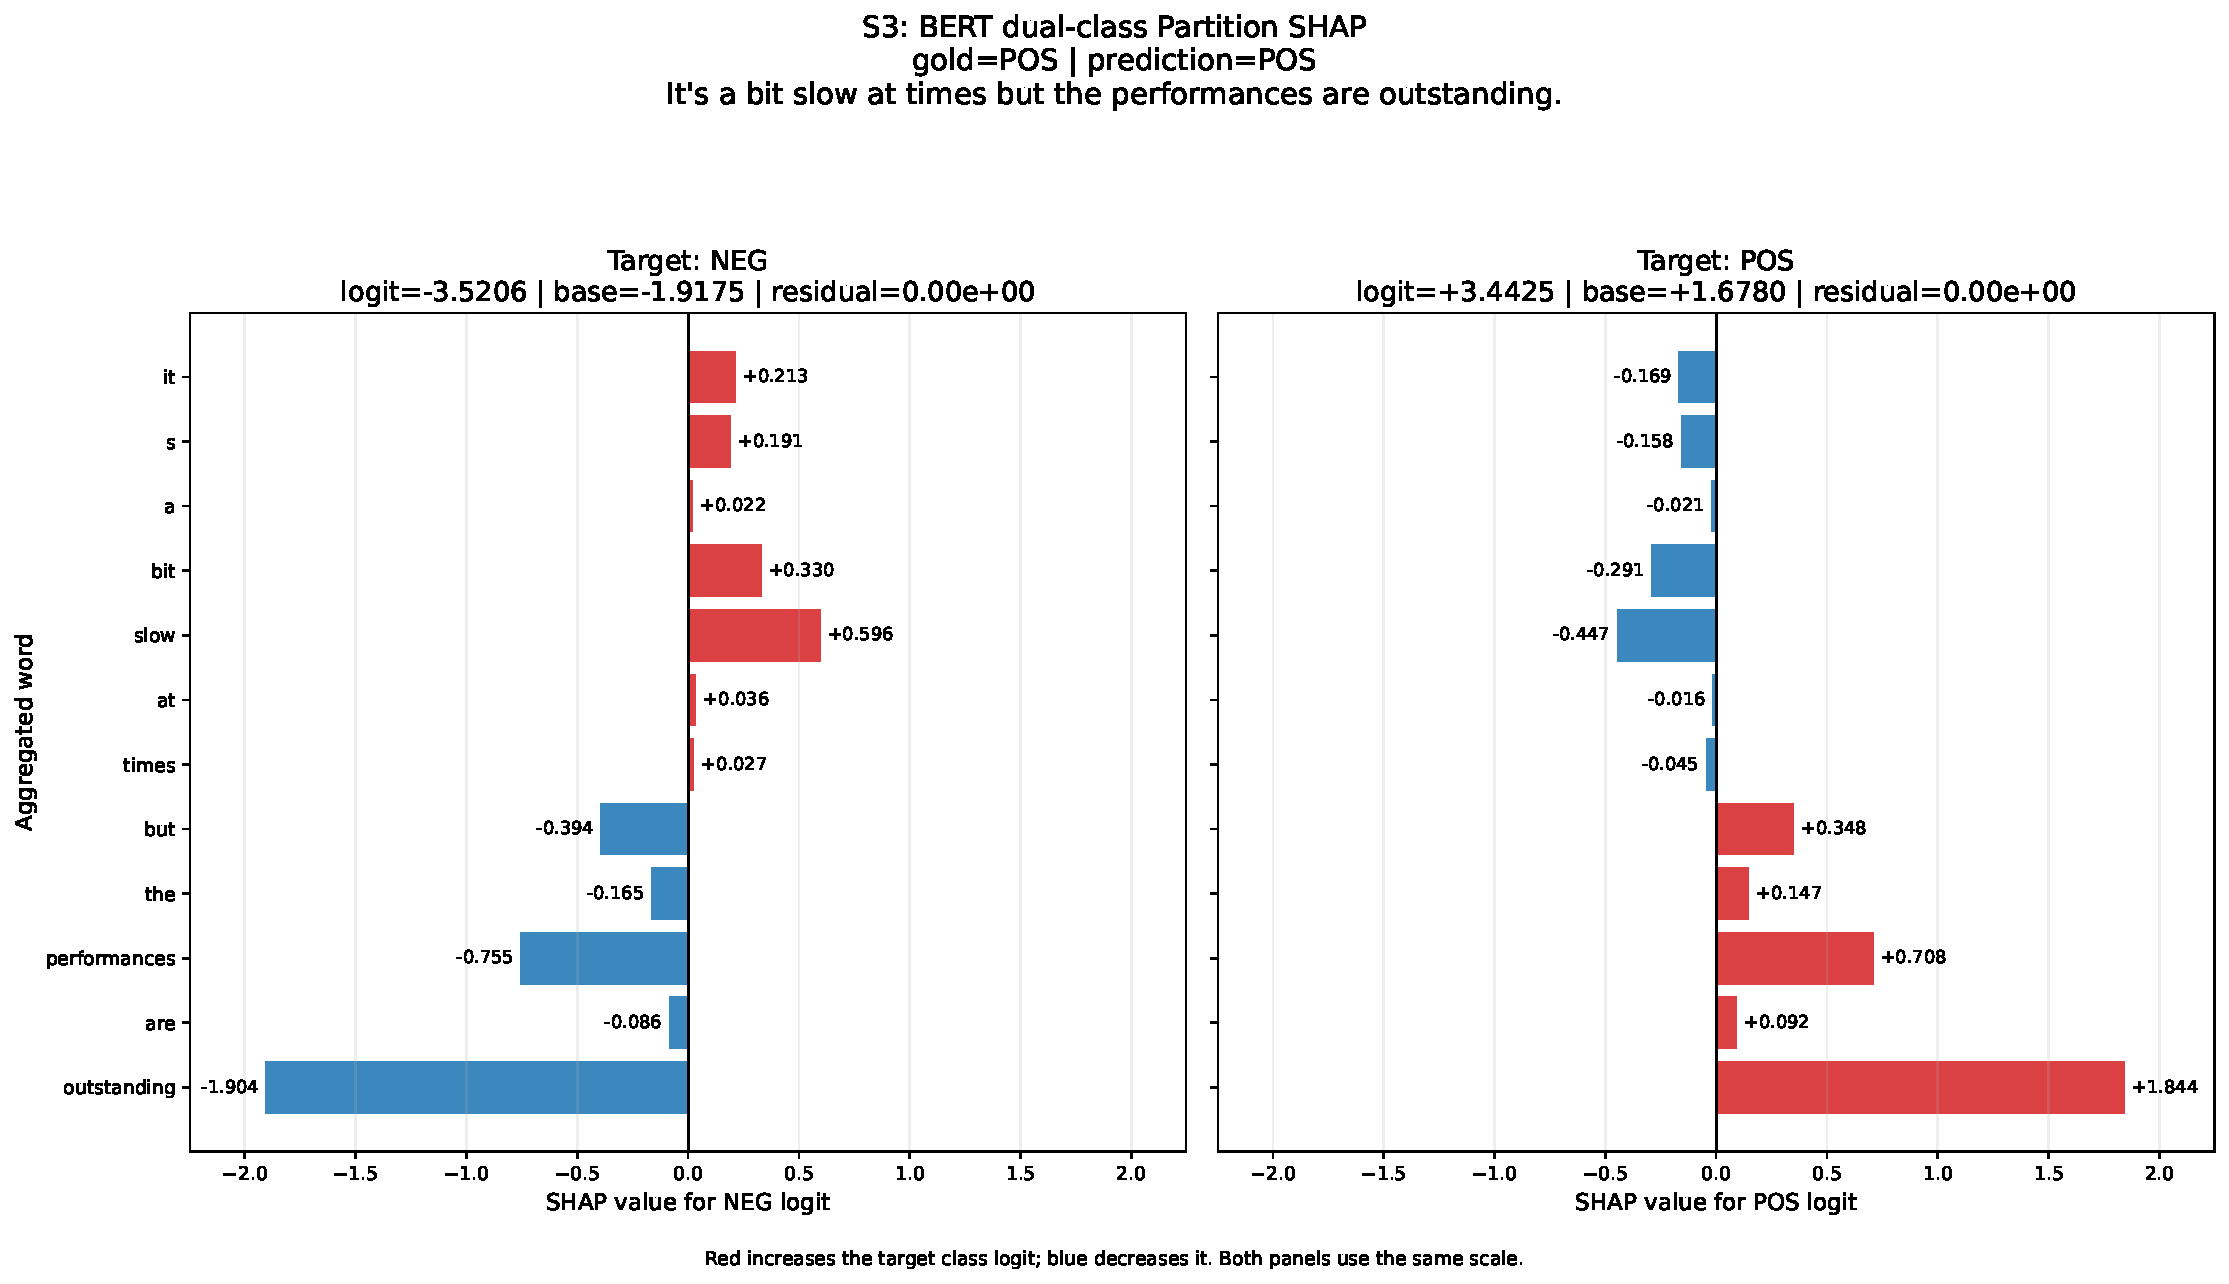
\includegraphics[width=\textwidth,height=0.3\textheight,keepaspectratio]{02_dual_class_bert_S1_S10/S3/S3_dual_class_word_bar.pdf}\\[3mm]
  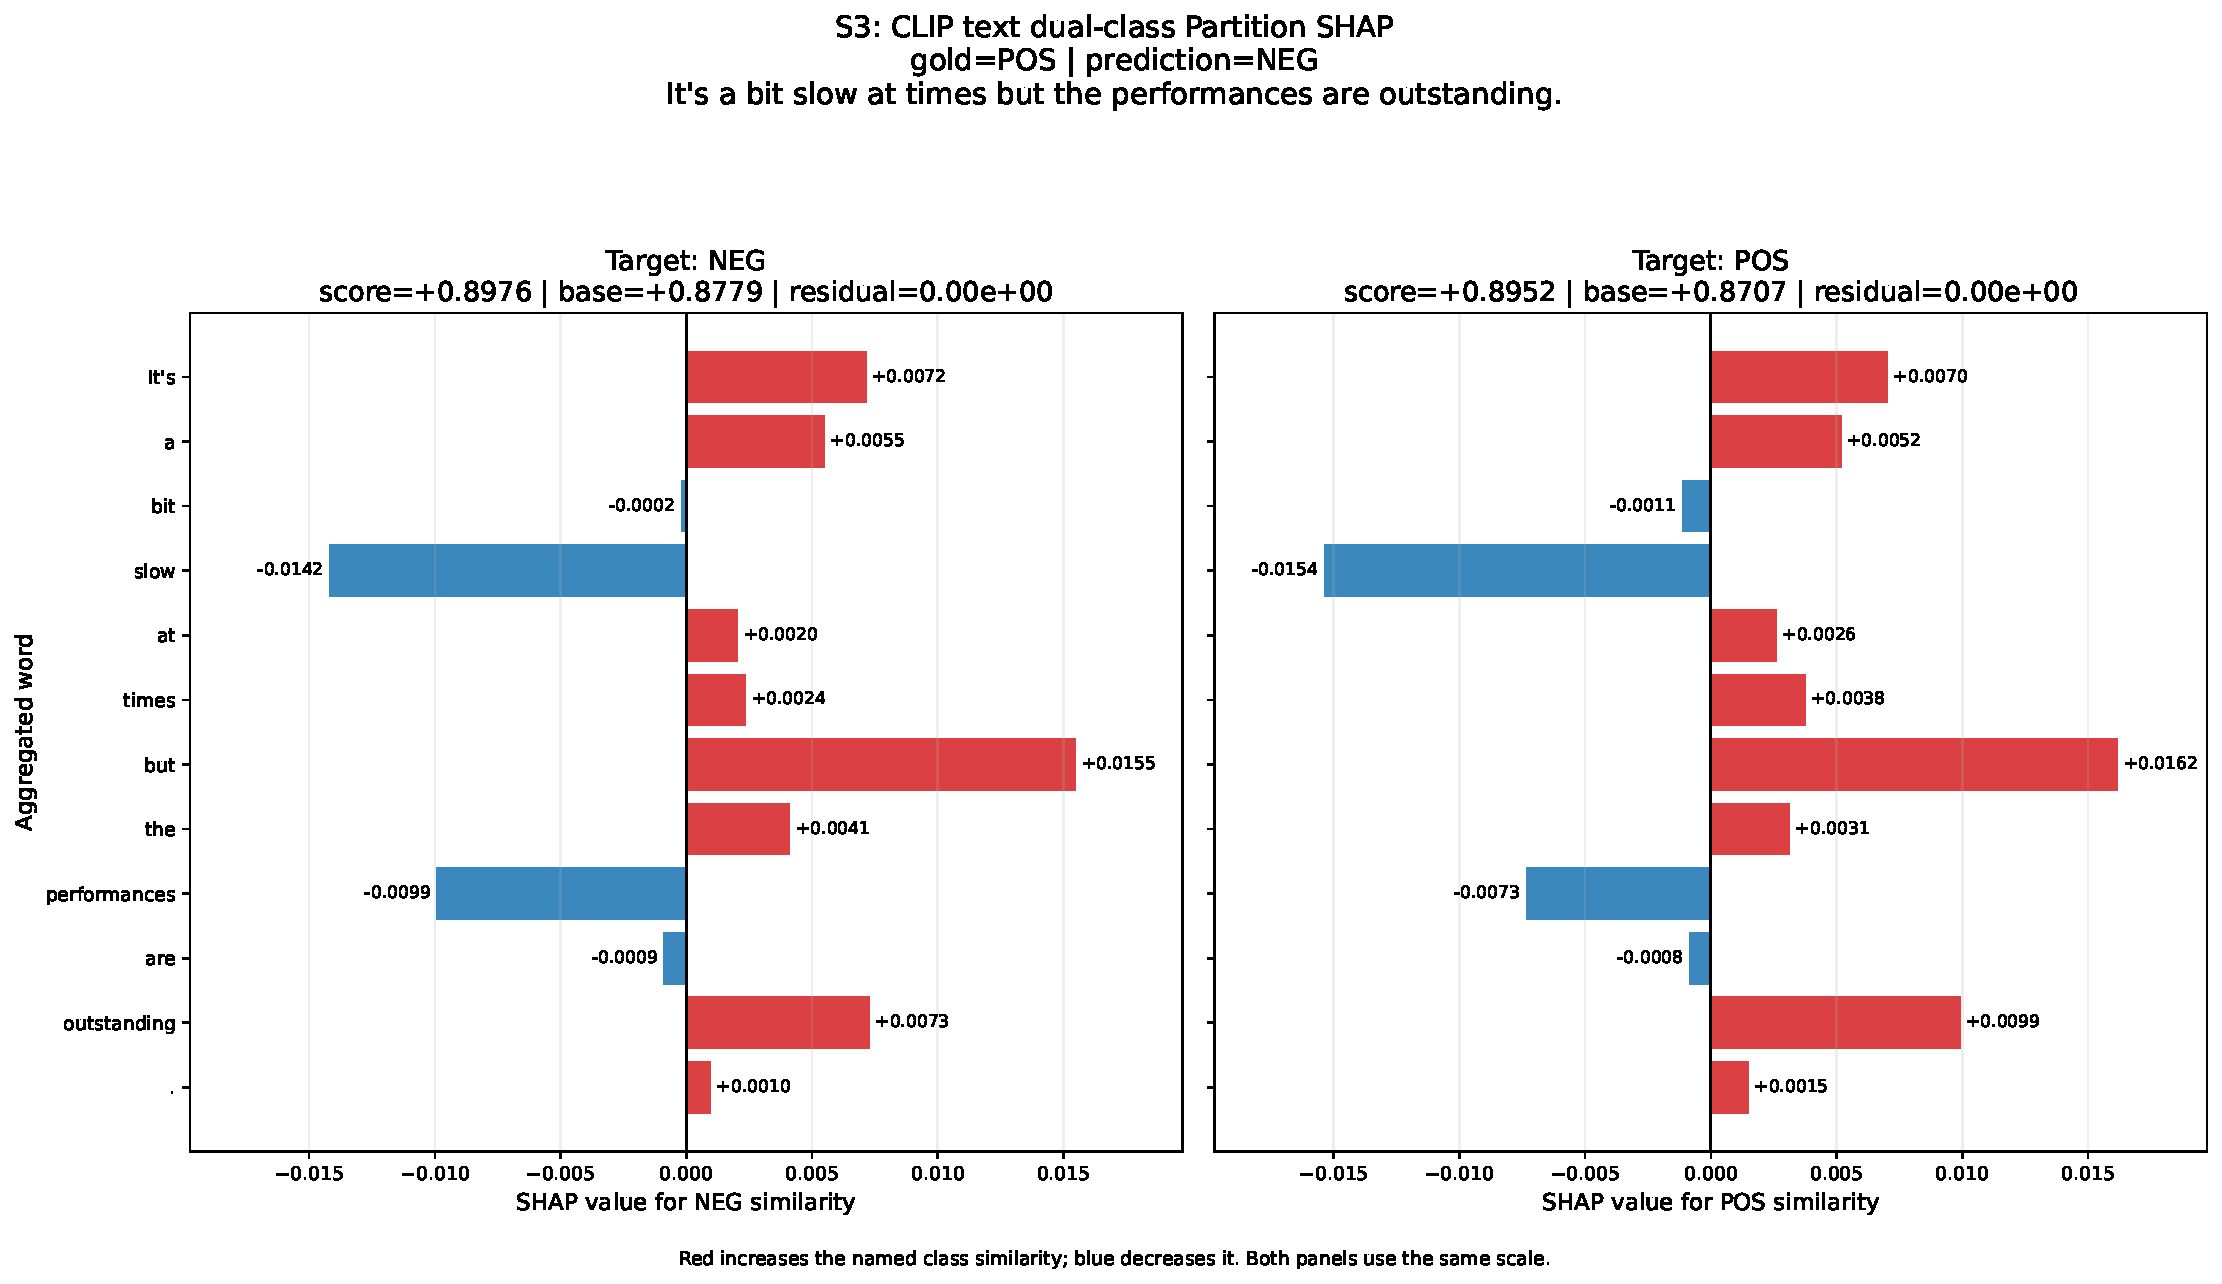
\includegraphics[width=\textwidth,height=0.3\textheight,keepaspectratio]{03_clip_text_shap_S1_S10/S3/S3_dual_class_word_bar.pdf}
  \caption[Word-level SHAP bars of BERT and CLIP text for sentence S3]{Sentence S3, ``It's a
           bit slow at times but the performances are outstanding.'' Top: BERT (correct,
           POS). Bottom: CLIP text (wrong, NEG). Each panel shows the SHAP values of one class
           output; red increases and blue decreases the named class.}
  \label{fig:s3-bars}
\end{figure}

\subsection{Two-class explanations of CLIP text on S1--S10}

CLIP text classifies nine of the ten sentences correctly; it fails on the contrastive
sentence S3 (Table~\ref{tab:s-predictions}). All explanations are again exactly additive.
The most striking difference to BERT is the size of the decisions: CLIP's margins lie
between 0.002 and 0.012 cosine units, while both class scores are around 0.90--0.98. In
other words, CLIP finds every sentence almost equally similar to the positive and the
negative prototype, and the decision is made by a very small difference.

This is also visible in the explanations (Figure~\ref{fig:s3-bars}, bottom). Unlike BERT,
CLIP's NEG and POS values mostly have the \emph{same} sign. Words that also occur in the
prompts, such as \emph{movie} in S2 or \emph{film} in S1, raise the similarity to
\emph{both} prototypes (for S2, \emph{movie} adds 0.050 to NEG and 0.059 to POS). They make
the sentence look like a movie review, but they do not decide its sentiment. Only the
margin column removes this shared part. After this correction the picture becomes more
familiar (Table~\ref{tab:s-words}): \emph{waste}, \emph{dull}, \emph{slow}, \emph{weak} and
\emph{disappointing} push towards NEG, and \emph{outstanding}, \emph{captivating},
\emph{charm} and \emph{entertaining} towards POS. In S3 CLIP does see \emph{outstanding} as
positive and \emph{slow} as negative, but the remaining words tip the tiny margin to NEG.

To compare the two models directly we correlated their word contributions to the margin.
Over S1--S10, the mean Spearman rank correlation is 0.37, on average 1.8 of the three most
important words are shared (Jaccard 0.46), and 59\,\% of the words receive the same sign.
The two models therefore agree on the most important sentiment words, but they rank the
remaining words quite differently. All plots are given in Appendix~\ref{app:clip-plots}.

\subsection{Faithfulness and plausibility on 500 sentences}\label{sec:text-results}

Before looking at the explanations, it helps to know how good the two classifiers are on
the 500 sentences (Table~\ref{tab:classification}). BERT, which was trained for this task,
reaches an accuracy of 93.6\,\%. CLIP text, used zero-shot through prompts, reaches
70.2\,\%. The SHAP explanations of both models passed the additivity check for all 500
sentences (largest residual $9.9\times10^{-6}$ logits for BERT and $5.7\times10^{-7}$ for
CLIP).

\begin{table}[H]
  \centering
  \caption{Classification results on the 500 SST-2 sentences (250 NEG, 250 POS).}
  \label{tab:classification}
  \small
  \begin{tabular}{@{}l r r r r@{}}
    \toprule
    Model & Accuracy & Macro-F1 & NEG recall & POS recall \\
    \midrule
    BERT (fine-tuned on SST-2) & 0.936 & 0.936 & 0.924 & 0.948 \\
    CLIP text (zero-shot)      & 0.702 & 0.702 & 0.688 & 0.716 \\
    \bottomrule
  \end{tabular}
\end{table}

Table~\ref{tab:text-metrics} shows the four explanation measures. BERT's explanations are
better on every measure.

\begin{table}[H]
  \centering
  \caption[Text explanation measures on 500 sentences]{Explanation measures for the
           POS$-$NEG margin SHAP values on the 500 sentences. Rationale measures use the SST
           word ratings as a proxy reference and are computed on the 468 sentences that
           contain at least one sentiment word.}
  \label{tab:text-metrics}
  \small
  \begin{tabular}{@{}l r r@{}}
    \toprule
    Metric & BERT & CLIP \\
    \midrule
    Comprehensiveness \up                & 0.7715 & 0.7049 \\
    Sufficiency \down                    & 0.2231 & 0.3307 \\
    Deletion AOPC \up                    & 0.8902 & $-0.3681$ \\
    Rationale precision (SST proxy) \up  & 0.4658 & 0.3277 \\
    Rationale recall (SST proxy) \up     & 0.6778 & 0.4886 \\
    Rationale F1 (SST proxy) \up         & 0.4935 & 0.3497 \\
    \bottomrule
  \end{tabular}
\end{table}

\paragraph{Comprehensiveness and sufficiency.} Deleting the top-ranked words removes on
average 77\,\% of a typical decision margin for BERT and 70\,\% for CLIP. Keeping only
those words loses 22\,\% of a typical margin for BERT and 33\,\% for CLIP. For both
models the explanations are clearly informative: a few words carry most of the decision.
BERT's explanations are somewhat more comprehensive and considerably more sufficient,
i.e.\ BERT's decision can be recovered better from the words SHAP selects. This extends the
observation of the previous report from ten sentences to 500. Table~\ref{tab:text-fractions}
shows that both measures behave as expected with the size of the selection:
comprehensiveness increases and sufficiency decreases the more words are selected.

\begin{table}[H]
  \centering
  \caption[Text measures at each cut-off]{Text measures at each cut-off (means over the 500
           sentences; rationale measures over 468 sentences). Mean $k$ is the average number
           of selected words; the normalized deletion drop is the per-cut-off term of the
           deletion AOPC.}
  \label{tab:text-fractions}
  \small
  \begin{tabular*}{\textwidth}{@{\extracolsep{\fill}} r r r r r r r r @{}}
    \toprule
    & & \multicolumn{2}{c}{Comprehensiveness \up} & \multicolumn{2}{c}{Sufficiency \down}
    & \multicolumn{2}{c}{Norm.\ deletion drop \up} \\
    \cmidrule(lr){3-4}\cmidrule(lr){5-6}\cmidrule(lr){7-8}
    Cut-off & Mean $k$ & BERT & CLIP & BERT & CLIP & BERT & CLIP \\
    \midrule
    10\,\% & 2.1 & 0.560 & 0.453 & 0.285 & 0.421 & 0.614 & $-1.693$ \\
    20\,\% & 3.8 & 0.724 & 0.640 & 0.270 & 0.400 & 0.888 & $-0.683$ \\
    30\,\% & 5.5 & 0.846 & 0.779 & 0.209 & 0.302 & 0.995 & 0.238 \\
    50\,\% & 8.6 & 0.956 & 0.948 & 0.128 & 0.200 & 1.064 & 0.665 \\
    \bottomrule
  \end{tabular*}

  \vspace{3mm}
  \begin{tabular*}{\textwidth}{@{\extracolsep{\fill}} r r r r r r r @{}}
    \toprule
    & \multicolumn{2}{c}{Rationale precision \up} & \multicolumn{2}{c}{Rationale recall \up}
    & \multicolumn{2}{c}{Rationale F1 \up} \\
    \cmidrule(lr){2-3}\cmidrule(lr){4-5}\cmidrule(lr){6-7}
    Cut-off & BERT & CLIP & BERT & CLIP & BERT & CLIP \\
    \midrule
    10\,\% & 0.604 & 0.381 & 0.460 & 0.284 & 0.490 & 0.305 \\
    20\,\% & 0.508 & 0.348 & 0.632 & 0.421 & 0.528 & 0.356 \\
    30\,\% & 0.426 & 0.314 & 0.753 & 0.545 & 0.511 & 0.374 \\
    50\,\% & 0.326 & 0.267 & 0.866 & 0.704 & 0.445 & 0.364 \\
    \bottomrule
  \end{tabular*}
\end{table}

\paragraph{Deletion AOPC.} For BERT, deleting the top-ranked words removes on average 89\,\%
of each sentence's own margin. At 50\,\% of the words the average drop is even slightly
larger than the margin itself (1.06), and 46\,\% of BERT's predictions flip to the other
class. For CLIP the mean is \emph{negative} ($-0.368$). This does not mean that CLIP's
explanations point the wrong way. The per-sentence normalization divides by the sentence's
own margin, and for the 73 CLIP sentences with a margin below 0.001 a tiny change in
similarity becomes a very large normalized value, in either direction. These few sentences
dominate the mean. The median deletion AOPC, which is not affected by them, is 0.70 for
CLIP and 0.67 for BERT. This is the reason why we normalized comprehensiveness and
sufficiency by the model's average margin instead: they use the same deletions as AOPC but
are not dominated by near-zero margins.

\paragraph{Rationale F1.} BERT's selected words agree clearly better with the human
sentiment ratings: 47\,\% of its selected words are sentiment words (CLIP 33\,\%), and it
finds 68\,\% of the sentiment words (CLIP 49\,\%). As expected, precision falls and recall
rises when more words are selected; the F1 score is highest at 20--30\,\% of the words for
both models. Two properties of the proxy reference should be kept in mind. First, it does
not capture sentiment that arises from context: in ``the film tries too hard to be funny'',
\emph{funny} counts as a sentiment word while \emph{tries too hard}, which carries the
negative judgment, does not. Second, a few mildly rated words such as \emph{out},
\emph{us} or \emph{life} fall just outside the neutral band and count as sentiment words.
The absolute F1 values are therefore not very meaningful on their own, but the comparison
between the two models is fair, because both are measured against the identical reference.

\subsection{Patch-level explanations of CLIP vision on I1--I10}

Figure~\ref{fig:vision-examples} shows two of the ten patch explanations; all ten are given
in Appendix~\ref{app:vision-plots}. In all images every patch received a non-negative value,
i.e.\ every visible region helps CLIP to keep its representation of the image. The values
are small (the largest patch value per image is between 0.020 and 0.053, while the gap
between the blurred and the original image is about 0.5), which shows that the
representation is spread over many patches. The largest values lie on the main object in
most images: on the kayak and paddler in I4, on the puppy's head in I5, on the child's face
in I10 and on the man's cap in I8. In I1, however, the highest value lies on the burning
stump in the lower right corner and not on the horse, which is the largest object in the
picture. A repeated run of I1 with 1,000 instead of 500 SHAP evaluations gave almost the
same patch values (Spearman correlation 0.98, same top patch), so these maps are stable
with respect to the evaluation budget.

\begin{figure}[htbp]
  \centering
  \begin{subfigure}{0.49\textwidth}\centering
    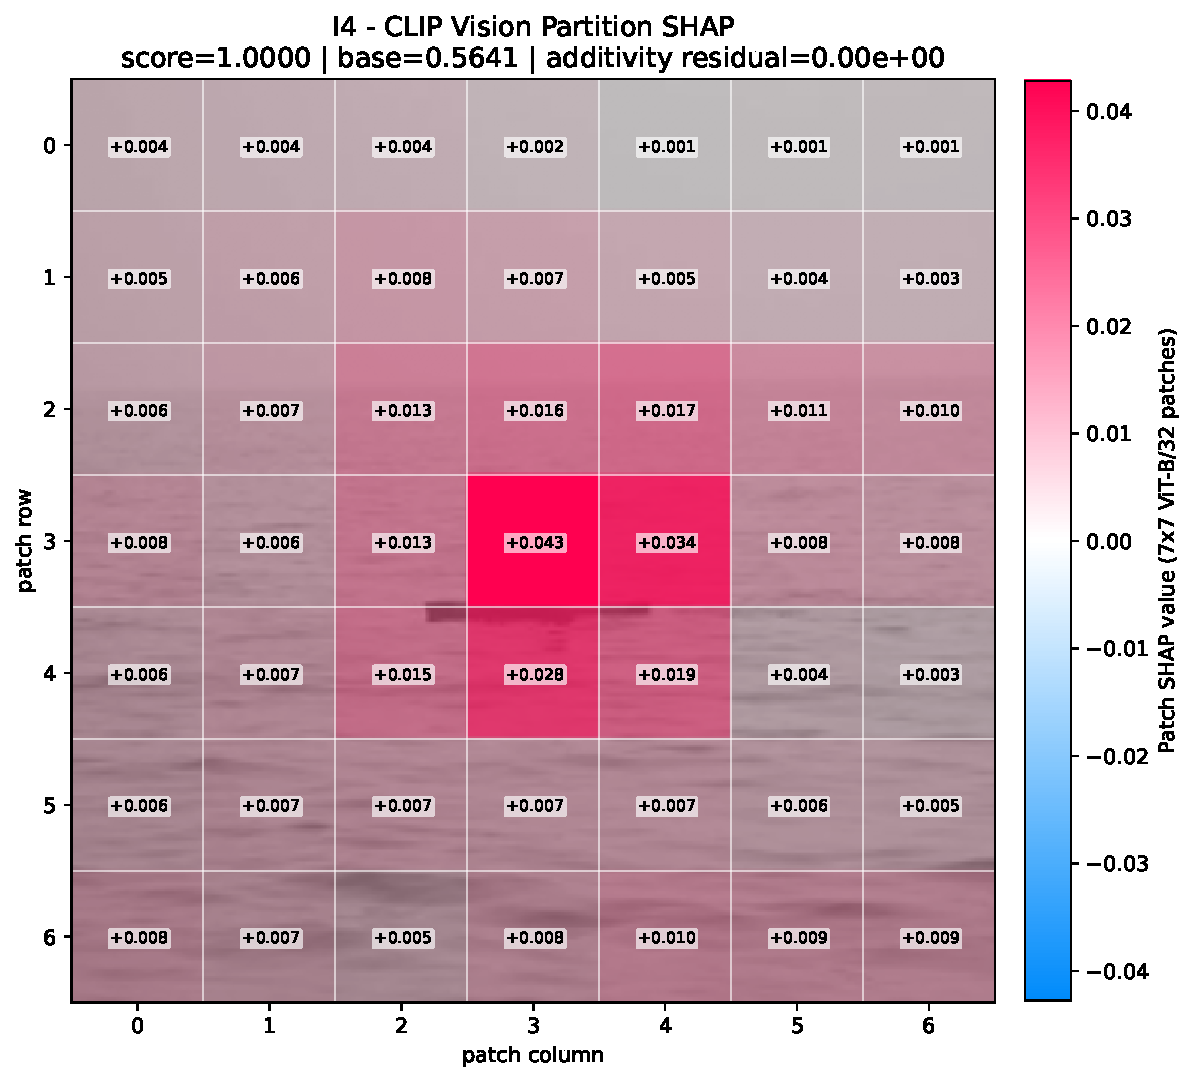
\includegraphics[width=\textwidth]{04_clip_vision_shap_I1_I10_patch_overlay_values/I4_SHAP_patch_overlay_values.pdf}
    \caption{I4: the top patch is on the kayak.}
  \end{subfigure}\hfill
  \begin{subfigure}{0.49\textwidth}\centering
    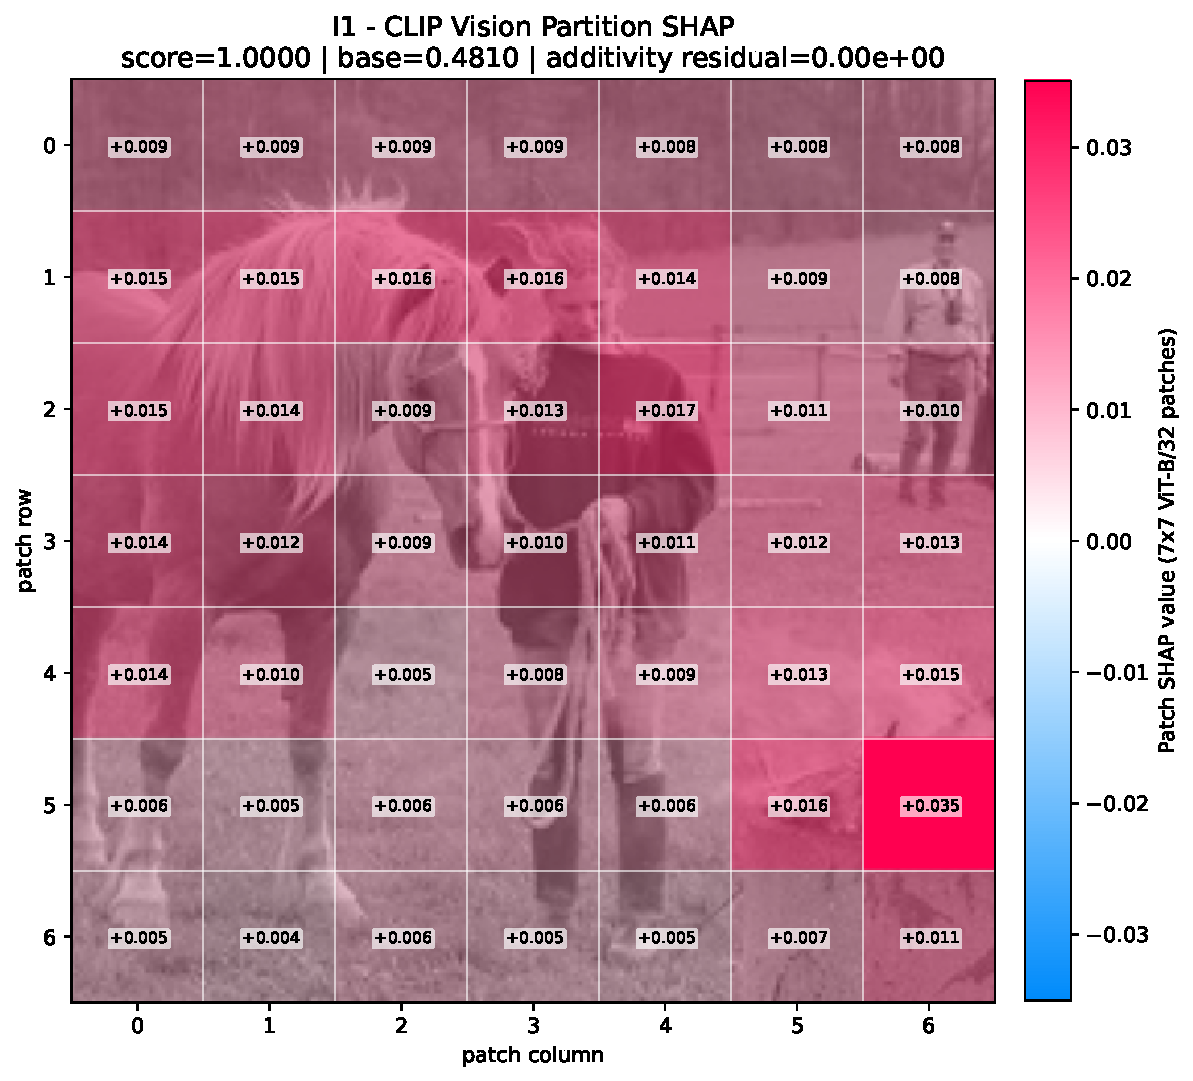
\includegraphics[width=\textwidth]{04_clip_vision_shap_I1_I10_patch_overlay_values/I1_SHAP_patch_overlay_values.pdf}
    \caption{I1: the top patch is on the burning stump.}
  \end{subfigure}
  \caption[Patch-level SHAP values of CLIP vision for I4 and I1]{Patch-level SHAP values of
           CLIP vision for two images. Each cell is one $32\times32$ ViT patch of the
           $224\times224$ input; darker red means a larger contribution to keeping the image
           embedding.}
  \label{fig:vision-examples}
\end{figure}

\subsection{Faithfulness and pointing game for CLIP vision}

Table~\ref{tab:vision-metrics} summarizes the four image measures and
Table~\ref{tab:vision-images} gives the values per image.

\begin{table}[H]
  \centering
  \caption{Explanation measures for CLIP vision (means over I1--I10).}
  \label{tab:vision-metrics}
  \small
  \begin{tabular}{@{}l r@{}}
    \toprule
    Metric & CLIP Vision \\
    \midrule
    Deletion AUC \down                     & 0.7109 \\
    Insertion AUC \up                      & 0.8492 \\
    AOPC \up                               & 0.1995 \\
    Pointing/localization accuracy \up     & 0.9000 \\
    \quad without pixel tolerance          & 0.7000 \\
    \bottomrule
  \end{tabular}
\end{table}

\begin{table}[H]
  \centering
  \caption[CLIP vision measures per image]{CLIP vision measures per image. ``Blurred'' is the
           similarity of the fully blurred image, i.e.\ the end of the deletion curve and the
           start of the insertion curve.}
  \label{tab:vision-images}
  \small
  \begin{tabular}{@{}l r r r r l c c@{}}
    \toprule
    Image & Blurred & DAUC \down & IAUC \up & AOPC \up & Target object & Hit (15 px) & Hit (0 px) \\
    \midrule
    I1  & 0.481 & 0.742 & 0.878 & 0.182 & horse                  & no  & no  \\
    I2  & 0.507 & 0.734 & 0.875 & 0.134 & people                 & yes & no  \\
    I3  & 0.471 & 0.768 & 0.890 & 0.156 & person                 & yes & yes \\
    I4  & 0.564 & 0.768 & 0.933 & 0.179 & kayak with paddler     & yes & yes \\
    I5  & 0.499 & 0.656 & 0.882 & 0.336 & dogs                   & yes & yes \\
    I6  & 0.296 & 0.637 & 0.764 & 0.208 & puppet-theatre cart    & yes & yes \\
    I7  & 0.445 & 0.686 & 0.806 & 0.193 & people (vendors)       & yes & yes \\
    I8  & 0.430 & 0.678 & 0.802 & 0.218 & person                 & yes & yes \\
    I9  & 0.408 & 0.765 & 0.830 & 0.156 & people (couple)        & yes & no  \\
    I10 & 0.420 & 0.676 & 0.832 & 0.233 & child                  & yes & yes \\
    \bottomrule
  \end{tabular}
\end{table}

\paragraph{Deletion and insertion.} Figure~\ref{fig:curves} shows the curves. Blurring the
single most important patch already lowers the mean similarity from 1 to about 0.92; after
one quarter of the patches it is about 0.82 and after half of them about 0.72. In the
insertion direction, restoring the single most important patch raises the similarity of the
blurred image from 0.45 to 0.56, and restoring the first quarter of the patches brings it
to about 0.78. Both curves therefore move fastest at the beginning, which is what we expect
when the ranking puts the important patches first. The deletion AUC of 0.71 must be read
together with the baseline: the deletion curve cannot fall below the similarity of the
fully blurred image (0.45 on average), so an area close to zero is impossible here. The
same holds for AOPC: blurring the top 10--50\,\% of the patches lowers the similarity by
0.20 on average, compared with a maximum possible drop of about 0.55.

\begin{figure}[htbp]
  \centering
  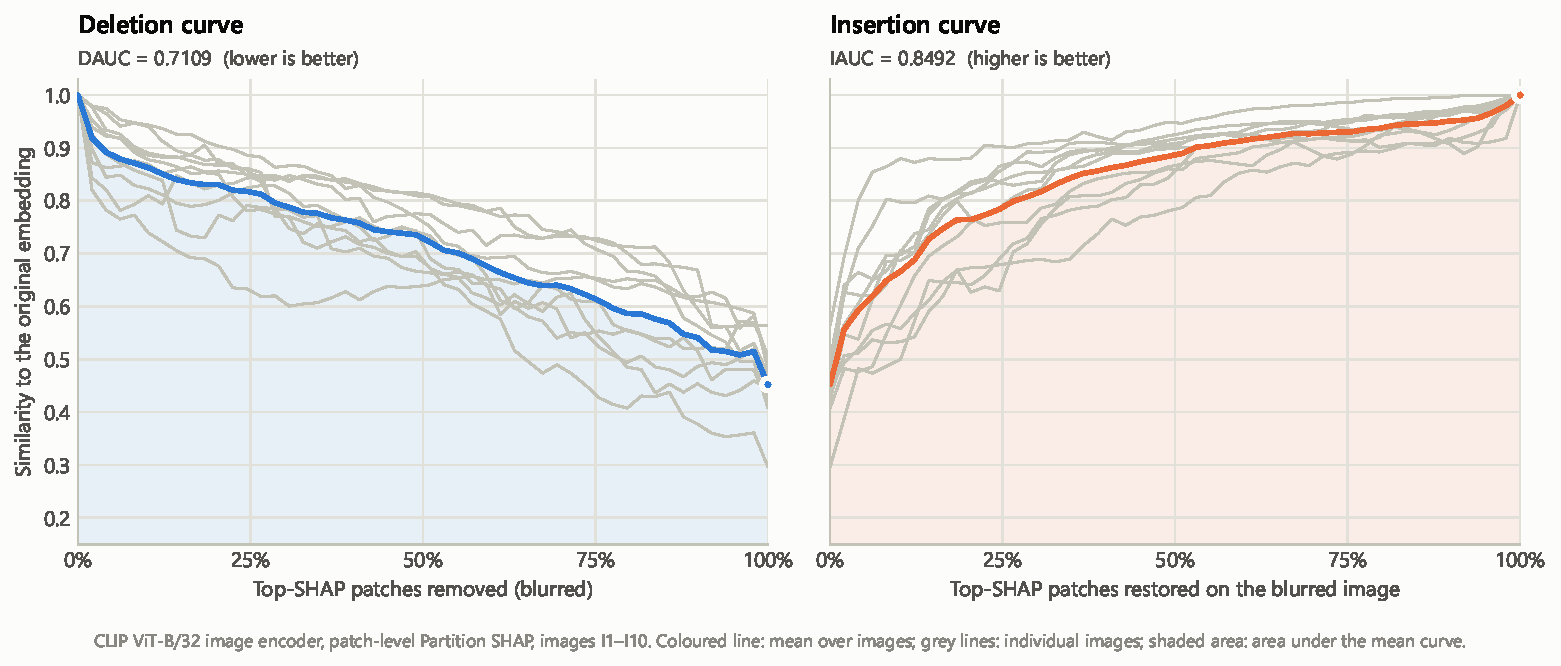
\includegraphics[width=\textwidth]{05_clip_vision_faithfulness_metrics/deletion_insertion_curves_mean.pdf}
  \caption[Deletion and insertion curves of CLIP vision]{Deletion (left) and insertion
           (right) curves of CLIP vision. Gray: individual images; colored: mean over the ten
           images; shaded: area under the mean curve. The per-image curves are shown in
           Appendix~\ref{app:extra}.}
  \label{fig:curves}
\end{figure}

\paragraph{Pointing game.} In 9 of the 10 images the center of the highest-ranked patch
lies on the annotated object (Figure~\ref{fig:pointing}). Two of these hits (I2 and I9)
are only within the 15-pixel tolerance: the point lies 10 and 12 pixels outside the box.
Without tolerance the accuracy is therefore 0.70. The clear miss is I1, where the top patch
lies on the fire. We should also note that the group boxes in I2 and I7 are large, which
makes a hit easier than for a small single object such as the fisherman in I3 or the couple
in I9.

\begin{figure}[htbp]
  \centering
  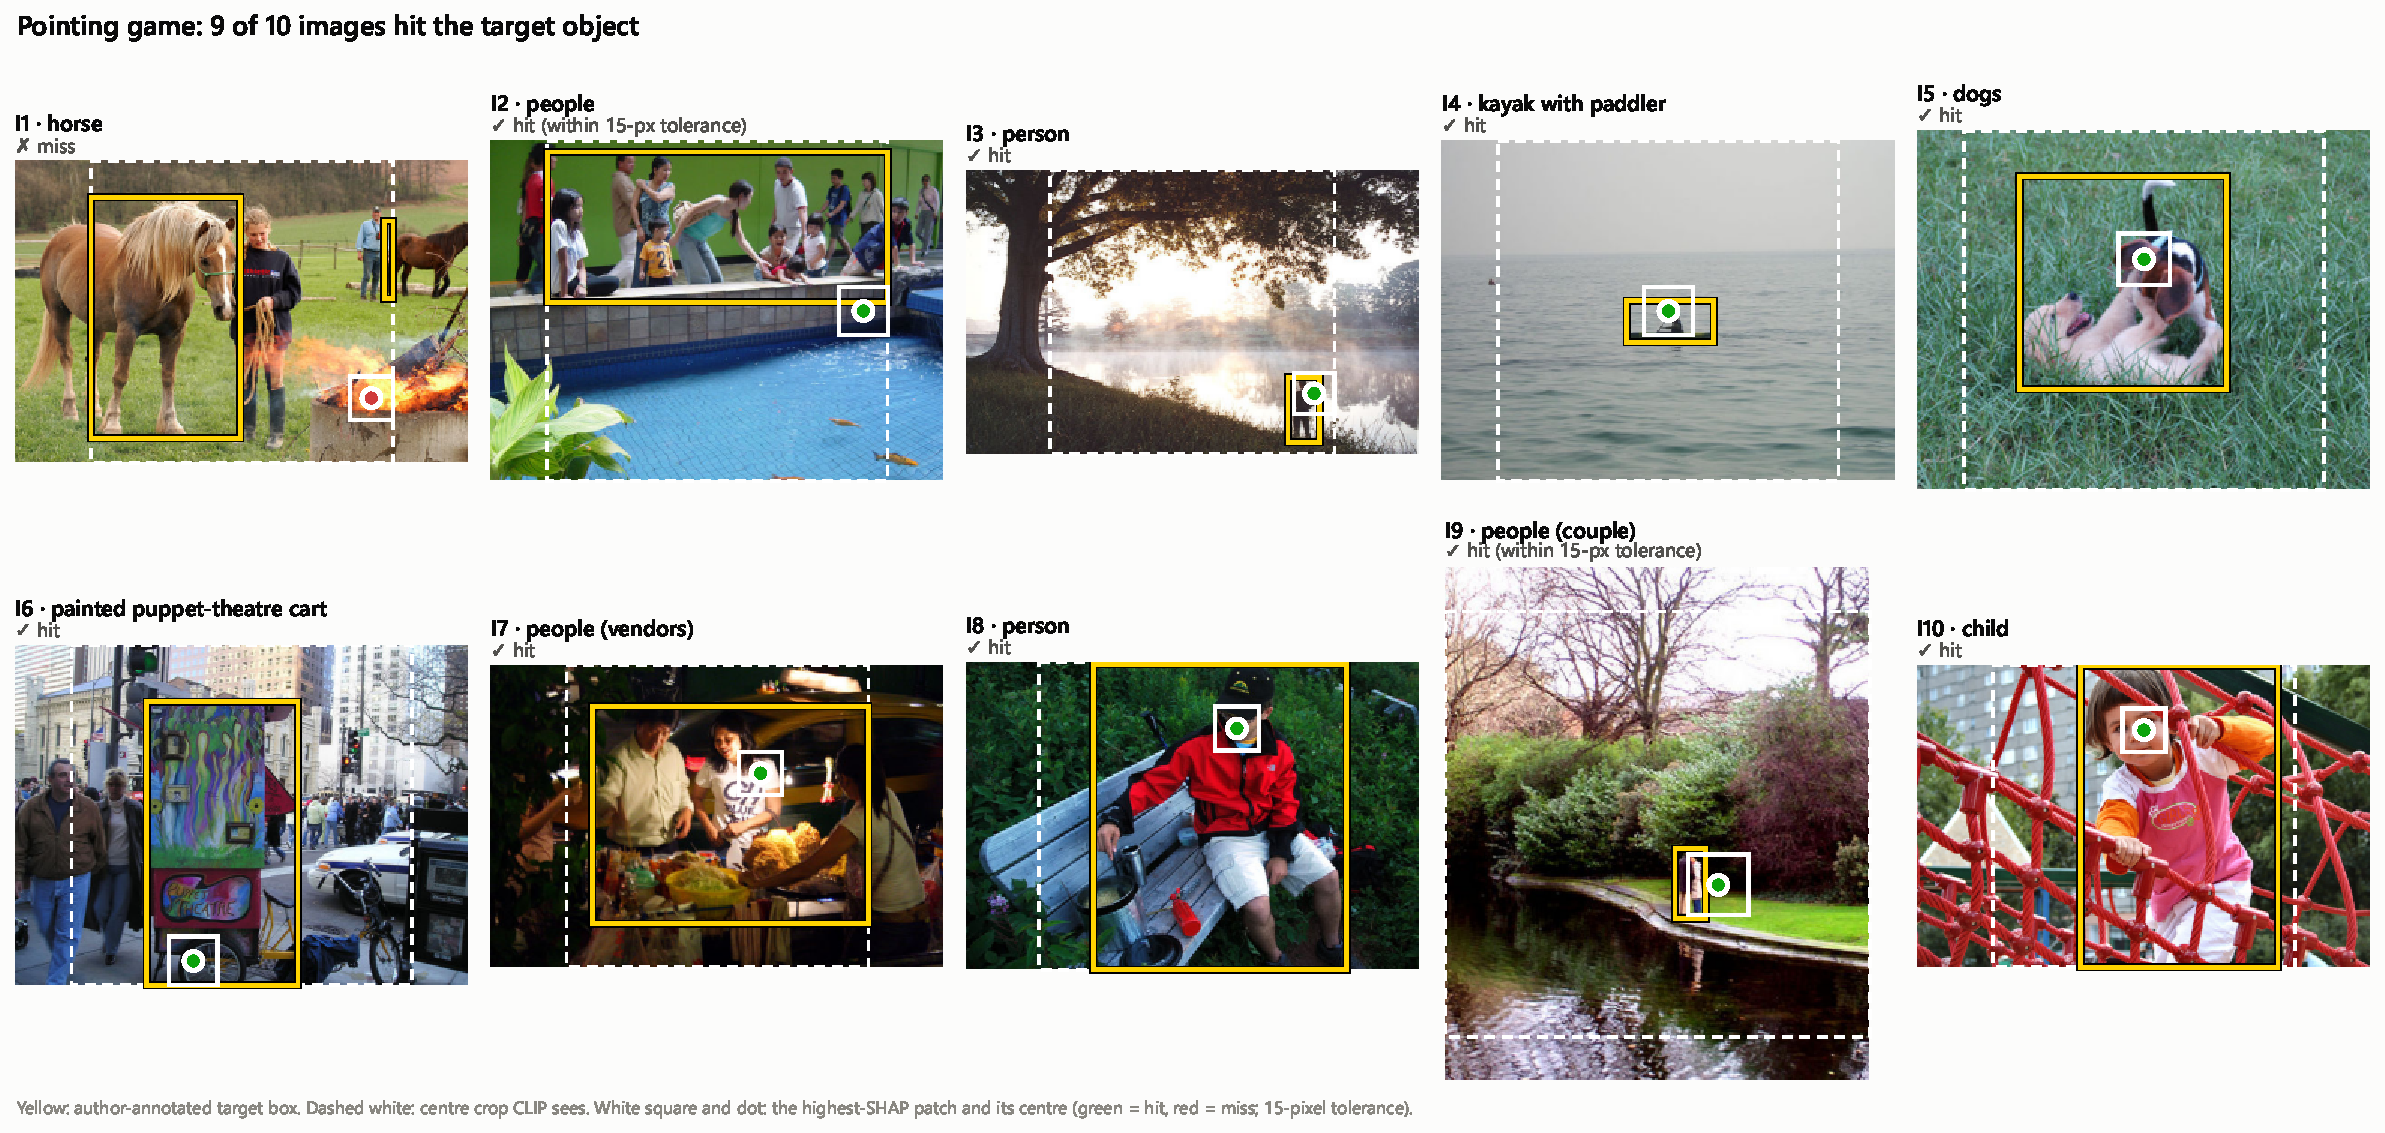
\includegraphics[width=\textwidth]{05_clip_vision_faithfulness_metrics/pointing_game.pdf}
  \caption[Pointing game for CLIP vision]{Pointing game. Yellow: annotated target box;
           dashed white: the center crop CLIP sees; white square and dot: the highest-ranked
           patch and its center (green = hit, red = miss).}
  \label{fig:pointing}
\end{figure}

% ======================================================================
\section{Discussion}\label{sec:discussion}

\paragraph{What the results tell us.} Across all experiments Partition SHAP produced
explanations that are internally consistent: every explanation reproduces the explained
model output, and the evaluation reproduced all stored scores. For BERT the explanations
are also convincing from the outside. The two-class explanations agree with the margin
explanation of the previous report and show that each word acts on both logits in
opposite directions (objective 1). On 500 sentences, removing the top-ranked words destroys
most of the decision while keeping them preserves most of it (objective 3), and the
selected words agree reasonably well with human word ratings (objective 4). The main
finding of the previous report therefore holds on a much larger set.

\paragraph{BERT versus CLIP text.} The explanations of CLIP text are weaker on every
measure (objectives 2--4), but we think this mostly reflects the model and not the
explanation method. CLIP was never trained for sentiment; with prompts it reaches 70\,\%
accuracy, and its decisions rest on very small differences between two large similarities.
In such a model, many words change both class scores together (for example words that
appear in the prompts), and the part that decides the sentiment is small. SHAP faithfully
reports this, which is why the CLIP explanations are less concentrated on sentiment words.
The comparison also taught us that the choice of normalization matters: with the
per-sentence normalization of the original AOPC, the mean for CLIP is negative and says
little about the explanations, while the same deletions normalized by the model's typical
margin give a clear and comparable result.

\paragraph{CLIP vision.} For images SHAP also produced faithful rankings (objective 5): the
curves change fastest for the first patches and the most important patch usually lies on the
main object. The explained score is, however, special. Because CLIP vision has no class
output, we explain how well the image keeps its own embedding. The most important regions
are then the regions that make the image recognizable as a whole, which often, but not
always, is the main object. I1 is a good example: the fire is small but visually very
distinctive, and CLIP apparently needs it to represent this particular image.

\paragraph{Limitations.} Several choices limit how far the numbers can be interpreted.
\begin{itemize}[leftmargin=*]
  \item \textbf{Masking baseline.} All SHAP values and all deletion measures depend on what a
        ``missing'' word or patch is: a \texttt{[MASK]} token, a deleted word or a blurred
        region. The models never saw such inputs during training. We used the same
        definition for explanation and evaluation, which keeps the comparison consistent,
        but a different baseline could give different values.
  \item \textbf{Partition approximation.} Partition SHAP computes Owen values with at most 500
        evaluations, not exact Shapley values. The stability check on I1 suggests that this
        budget is sufficient, but we checked it only for one image.
  \item \textbf{Proxy references.} Rationale F1 uses context-free word ratings instead of
        sentence-specific human rationales, and the pointing game uses boxes that we
        annotated ourselves. Both are reasonable substitutes, but they are not benchmark
        ground truth, and we report them as such.
  \item \textbf{Small qualitative sets.} S1--S10 and I1--I10 are ten examples each. They are
        useful to understand the explanations, but the vision measures in particular rest on
        ten images only.
  \item \textbf{Different settings across experiments.} Experiments A/B and C use different
        masking and different CLIP prompts, so their SHAP values are not directly
        comparable. We therefore only compare BERT and CLIP \emph{within} one experiment.
  \item \textbf{No uncertainty estimates.} We report plain averages without confidence
        intervals, as required for this part of the project. Small differences, such as the
        comprehensiveness gap of 0.07, should therefore not be over-interpreted.
\end{itemize}

\paragraph{What we learned.} Working on this project, we found that an explanation method
is only half of the work; the other half is making sure the numbers mean what we think
they mean. Checking additivity, re-scoring the stored inputs and hashing the source
folders caught several subtle problems during development, for example when a quantity we
had quoted turned out to be a difference between two metrics. We also learned to be careful
with normalization and with references that only approximate human judgment.

% ======================================================================
\section{Conclusion}\label{sec:conclusion}

We extended our previous SHAP analysis of BERT to two-class explanations, to the text and
vision encoders of CLIP, and to a quantitative evaluation with established measures. For
BERT on SST-2 the explanations identify the expected sentiment words, are faithful
(comprehensiveness 0.772, sufficiency 0.223, deletion AOPC 0.890) and agree with human word
ratings (rationale F1 0.494 with the SST proxy reference). For CLIP text used as a
zero-shot sentiment classifier, the explanations are less faithful and less plausible
(comprehensiveness 0.705, sufficiency 0.331, rationale F1 0.350), which matches its weaker
classification (70\,\% vs.\ 94\,\% accuracy) and its very small decision margins. For CLIP
vision the patch rankings are faithful (deletion AUC 0.711, insertion AUC 0.849, AOPC 0.199)
and the most important patch lies on the main object in 9 of 10 images.

Several extensions would make the results stronger: sentence-level human rationales (for
example from the ERASER movie review data) instead of the lexical proxy, images with
official bounding boxes (for example from COCO or PASCAL VOC), a class-specific target for
CLIP vision such as the similarity to a caption, other masking baselines, and confidence
intervals for all measures. A comparison with other attribution methods such as Integrated
Gradients would show how much of our findings is specific to SHAP.

% ======================================================================
\begin{thebibliography}{99}

\bibitem{lundberg2017}
S.~M. Lundberg and S.-I. Lee.
A unified approach to interpreting model predictions.
In \emph{Advances in Neural Information Processing Systems 30 (NeurIPS)}, 2017.

\bibitem{shapdocs}
SHAP documentation: Partition explainer.
\url{https://shap.readthedocs.io/}, accessed September 2026.

\bibitem{devlin2019}
J.~Devlin, M.-W. Chang, K.~Lee, and K.~Toutanova.
BERT: Pre-training of deep bidirectional transformers for language understanding.
In \emph{Proceedings of NAACL-HLT}, pages 4171--4186, 2019.

\bibitem{morris2020}
J.~Morris, E.~Lifland, J.~Y. Yoo, J.~Grigsby, D.~Jin, and Y.~Qi.
TextAttack: A framework for adversarial attacks, data augmentation, and adversarial
training in NLP.
In \emph{Proceedings of EMNLP: System Demonstrations}, pages 119--126, 2020.

\bibitem{socher2013}
R.~Socher, A.~Perelygin, J.~Wu, J.~Chuang, C.~D. Manning, A.~Ng, and C.~Potts.
Recursive deep models for semantic compositionality over a sentiment treebank.
In \emph{Proceedings of EMNLP}, pages 1631--1642, 2013.

\bibitem{wang2019}
A.~Wang, A.~Singh, J.~Michael, F.~Hill, O.~Levy, and S.~R. Bowman.
GLUE: A multi-task benchmark and analysis platform for natural language understanding.
In \emph{Proceedings of ICLR}, 2019.

\bibitem{radford2021}
A.~Radford, J.~W. Kim, C.~Hallacy, A.~Ramesh, G.~Goh, S.~Agarwal, G.~Sastry, A.~Askell,
P.~Mishkin, J.~Clark, G.~Krueger, and I.~Sutskever.
Learning transferable visual models from natural language supervision.
In \emph{Proceedings of ICML}, pages 8748--8763, 2021.

\bibitem{dosovitskiy2021}
A.~Dosovitskiy, L.~Beyer, A.~Kolesnikov, D.~Weissenborn, X.~Zhai, T.~Unterthiner,
M.~Dehghani, M.~Minderer, G.~Heigold, S.~Gelly, J.~Uszkoreit, and N.~Houlsby.
An image is worth 16x16 words: Transformers for image recognition at scale.
In \emph{Proceedings of ICLR}, 2021.

\bibitem{deyoung2020}
J.~DeYoung, S.~Jain, N.~F. Rajani, E.~Lehman, C.~Xiong, R.~Socher, and B.~C. Wallace.
ERASER: A benchmark to evaluate rationalized NLP models.
In \emph{Proceedings of ACL}, pages 4443--4458, 2020.

\bibitem{samek2017}
W.~Samek, A.~Binder, G.~Montavon, S.~Lapuschkin, and K.-R. M\"uller.
Evaluating the visualization of what a deep neural network has learned.
\emph{IEEE Transactions on Neural Networks and Learning Systems}, 28(11):2660--2673, 2017.

\bibitem{petsiuk2018}
V.~Petsiuk, A.~Das, and K.~Saenko.
RISE: Randomized input sampling for explanation of black-box models.
In \emph{Proceedings of BMVC}, 2018.

\bibitem{zhang2018}
J.~Zhang, S.~A. Bargal, Z.~Lin, J.~Brandt, X.~Shen, and S.~Sclaroff.
Top-down neural attention by excitation backprop.
\emph{International Journal of Computer Vision}, 126(10):1084--1102, 2018.

\end{thebibliography}

% ======================================================================
\clearpage
\appendix

\section{Qualitative sentence set}\label{app:sentences}

\begin{table}[H]
  \centering
  \caption{Complete qualitative sentence set used in experiments A and B.}
  \label{tab:sentences}
  \small
  \begin{tabularx}{\textwidth}{@{}l l Y@{}}
    \toprule
    ID & Gold & Sentence \\
    \midrule
    S1  & POS & The film is a beautiful and moving portrait of human resilience. \\
    S2  & NEG & This movie is an absolute waste of time and money. \\
    S3  & POS & It's a bit slow at times but the performances are outstanding. \\
    S4  & NEG & A dull, tedious and completely forgettable experience. \\
    S5  & POS & The direction is inspired and the acting is nothing short of brilliant. \\
    S6  & POS & A masterpiece of storytelling with breathtaking visuals and emotion. \\
    S7  & NEG & Painfully boring and utterly devoid of any originality or charm. \\
    S8  & POS & The screenplay is weak but the lead actor delivers a captivating turn. \\
    S9  & NEG & A hollow and disappointing sequel that betrays everything the original stood for. \\
    S10 & POS & Funny, heartfelt and endlessly entertaining from beginning to end. \\
    \bottomrule
  \end{tabularx}
\end{table}

\section{CLIP text prompt families}\label{app:prompts}

\begin{table}[H]
  \centering
  \caption{Prompts used to build the CLIP text prototypes.}
  \label{tab:prompts}
  \small
  \begin{tabularx}{\textwidth}{@{}l Y Y@{}}
    \toprule
    Experiment & NEG prompts & POS prompts \\
    \midrule
    B (S1--S10) &
      This movie is terrible. / I hated this movie. / This is a bad film. / The film was
      disappointing. / This is a negative movie review. &
      This movie is excellent. / I loved this movie. / This is a good film. / The film was
      enjoyable. / This is a positive movie review. \\
    \midrule
    C (500 sentences) &
      This is a negative review. / This movie is terrible. / The film was disappointing. /
      The reviewer disliked the film. / This film left a bad impression. / The overall
      judgement is negative. / This was an unenjoyable experience. / I would not recommend
      this film. &
      This is a positive review. / This movie is excellent. / The film was satisfying. /
      The reviewer liked the film. / This film left a good impression. / The overall
      judgement is positive. / This was an enjoyable experience. / I would recommend this
      film. \\
    \bottomrule
  \end{tabularx}
\end{table}

\section{Target boxes for the pointing game}\label{app:boxes}

Coordinates are pixels of the original image ($x_0,y_0$ = top left, $x_1,y_1$ = bottom
right). The boxes were drafted without looking at the SHAP maps and approved on
30 September 2026; for the evaluation they are clipped to the center crop CLIP sees.

\begin{table}[H]
  \centering
  \caption{Author-annotated target boxes.}
  \label{tab:boxes}
  \small
  \begin{tabularx}{\textwidth}{@{}l l r r r r Y@{}}
    \toprule
    Image & Target & $x_0$ & $y_0$ & $x_1$ & $y_1$ & Note \\
    \midrule
    I1  & horse                       & 8   & 40  & 248 & 306 & main horse \\
    I1  & horse                       & 407 & 66  & 500 & 152 & background horse, mostly outside the crop \\
    I2  & people                      & 25  & 12  & 500 & 178 & one box around the group at the pool edge \\
    I3  & person                      & 355 & 228 & 390 & 300 & man fishing; rest is landscape \\
    I4  & kayak with paddler          & 204 & 176 & 300 & 222 & \\
    I5  & dogs                        & 90  & 40  & 273 & 228 & both puppies \\
    I6  & painted puppet-theatre cart & 145 & 62  & 312 & 375 & booth with wheels \\
    I7  & people (vendors)            & 112 & 45  & 482 & 285 & three people at the stall \\
    I8  & person                      & 140 & 2   & 420 & 339 & man in the red jacket \\
    I9  & people (couple)             & 224 & 274 & 254 & 342 & couple by the pond \\
    I10 & child                       & 180 & 0   & 398 & 333 & child on the rope net \\
    \bottomrule
  \end{tabularx}
\end{table}

\section{Additional vision results}\label{app:extra}

\begin{figure}[H]
  \centering
  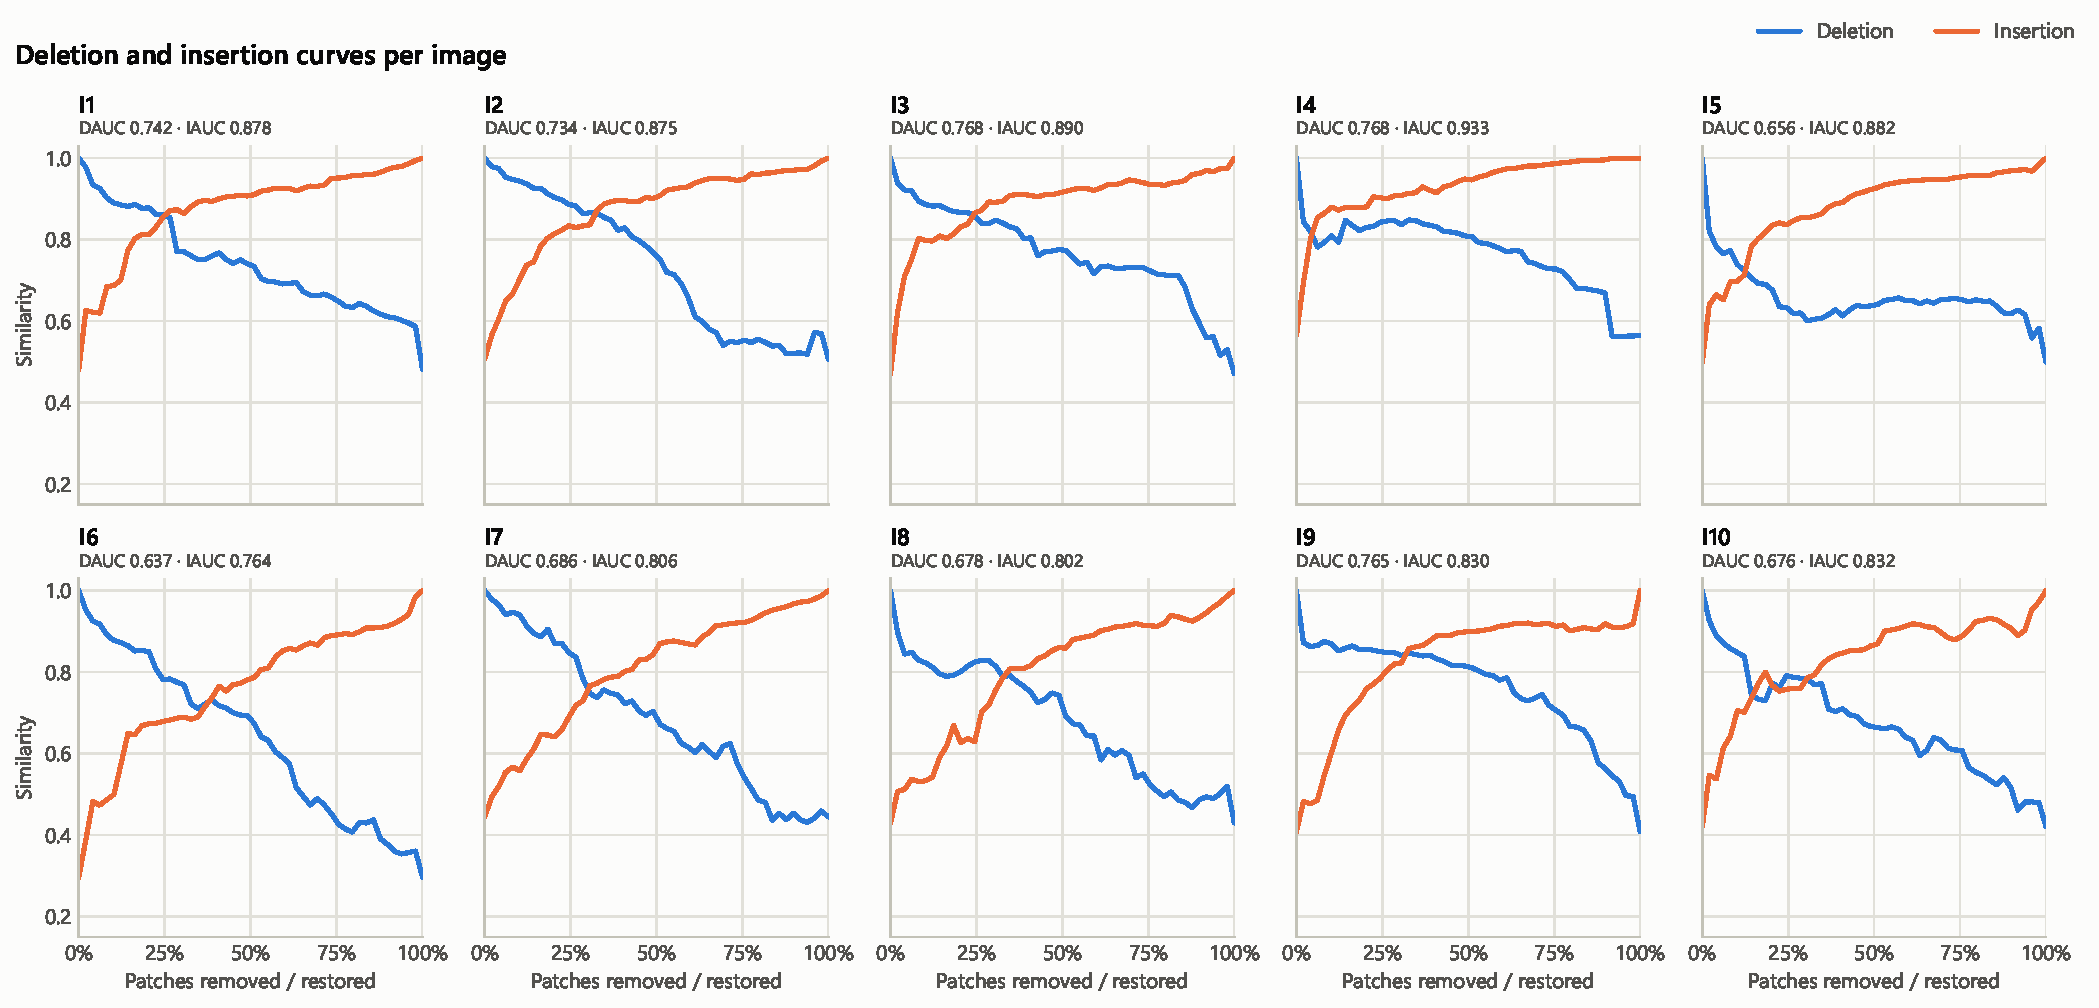
\includegraphics[width=\textwidth]{05_clip_vision_faithfulness_metrics/deletion_insertion_curves_per_image.pdf}
  \caption{Deletion and insertion curves for each image.}
  \label{fig:curves-per-image}
\end{figure}

\section{Reproducibility record}\label{app:repro}

\begin{table}[H]
  \centering
  \caption{Where the results of this report come from.}
  \label{tab:repro}
  \small
  \begin{tabularx}{\textwidth}{@{}l Y Y@{}}
    \toprule
    Part & Project folder & Report material \\
    \midrule
    A & \texttt{bert\_shap/dual\_class\_bert} (run \texttt{bert\_dual\_20\_curated}) &
        \texttt{02\_dual\_class\_bert\_S1\_S10} \\
    B & \texttt{clip\_text\_shap} (run \texttt{clip\_text\_dual\_20\_curated}) &
        \texttt{03\_clip\_text\_shap\_S1\_S10} \\
    C & \texttt{bert\_clip\_partition\_shap\_500} (SHAP values);
        \texttt{bert\_clip\_shap\_faithfulness\_metrics} (measures) &
        \texttt{01\_bert\_clip\_faithfulness\_metrics} \\
    D & \texttt{clip\_vision\_shap} (run \texttt{clip\_vision\_i1\_i10});
        \texttt{clip\_vision\_shap\_faithfulness\_metrics} (measures, boxes) &
        \texttt{04\_clip\_vision\_shap\_I1\_I10\_\allowbreak patch\_overlay\_values},
        \texttt{05\_clip\_vision\_\allowbreak faithfulness\_metrics} \\
    \bottomrule
  \end{tabularx}
\end{table}

Settings shared by all SHAP runs: Partition explainer, at most 500 model evaluations per
sentence or image, batch size 32, seed 42. BERT maximum length 128 tokens, CLIP text
maximum length 77 tokens, CLIP vision input $224\times224$ with a $128\times128$ box blur.
No model was trained or fine-tuned in this project. The evaluation projects contain a
\texttt{README.md} with all definitions and checks, a \texttt{checks.json} with every
verification result, and a batch file that re-runs the evaluation and its tests (23 tests
for the text measures, 13 for the image measures).

% ----------------------------------------------------------------------
\clearpage
\section{Complete BERT sentence-level plots}\label{app:bert-plots}

Each page shows the five plots of one sentence. In the word bars and matrices, red
increases and blue decreases the named class logit. The summary matrix reports the logits,
probabilities, base values, the sum of the SHAP values, the reconstructed logits and the
additivity residual.

\sentenceplots[0.84]{02_dual_class_bert_S1_S10}{S1}{BERT}{bert}
\sentenceplots{02_dual_class_bert_S1_S10}{S2}{BERT}{bert}
\sentenceplots{02_dual_class_bert_S1_S10}{S3}{BERT}{bert}
\sentenceplots{02_dual_class_bert_S1_S10}{S4}{BERT}{bert}
\sentenceplots{02_dual_class_bert_S1_S10}{S5}{BERT}{bert}
\sentenceplots{02_dual_class_bert_S1_S10}{S6}{BERT}{bert}
\sentenceplots{02_dual_class_bert_S1_S10}{S7}{BERT}{bert}
\sentenceplots{02_dual_class_bert_S1_S10}{S8}{BERT}{bert}
\sentenceplots{02_dual_class_bert_S1_S10}{S9}{BERT}{bert}
\sentenceplots{02_dual_class_bert_S1_S10}{S10}{BERT}{bert}

\section{Complete CLIP text sentence-level plots}\label{app:clip-plots}

Each page shows the five plots of one sentence. The values explain the cosine similarity
to the NEG and POS prompt prototypes; the summary matrix reports the similarities, base
values, the sum of the SHAP values, the reconstructed scores and the additivity residual.

\sentenceplots[0.84]{03_clip_text_shap_S1_S10}{S1}{CLIP text}{clip}
\sentenceplots{03_clip_text_shap_S1_S10}{S2}{CLIP text}{clip}
\sentenceplots{03_clip_text_shap_S1_S10}{S3}{CLIP text}{clip}
\sentenceplots{03_clip_text_shap_S1_S10}{S4}{CLIP text}{clip}
\sentenceplots{03_clip_text_shap_S1_S10}{S5}{CLIP text}{clip}
\sentenceplots{03_clip_text_shap_S1_S10}{S6}{CLIP text}{clip}
\sentenceplots{03_clip_text_shap_S1_S10}{S7}{CLIP text}{clip}
\sentenceplots{03_clip_text_shap_S1_S10}{S8}{CLIP text}{clip}
\sentenceplots{03_clip_text_shap_S1_S10}{S9}{CLIP text}{clip}
\sentenceplots{03_clip_text_shap_S1_S10}{S10}{CLIP text}{clip}

\section{Complete CLIP vision patch-level plots}\label{app:vision-plots}

Each figure shows the $7\times7$ patch SHAP values over the $224\times224$ input that CLIP
sees, with the value printed in each patch. The title reports the score of the original
image (1), the base value (the fully blurred image) and the additivity residual.

\visionpair[0.86]{I1}{I2}
\visionpair{I3}{I4}
\visionpair{I5}{I6}
\visionpair{I7}{I8}
\visionpair{I9}{I10}

\end{document}
